\documentclass[10pt,journal,compsoc]{IEEEtran}

\usepackage[T1]{fontenc}
\usepackage[utf8]{inputenc}

\usepackage{acronym} % \ac[p], \acl[p], \acs[p], \acf[p]

\usepackage[nocompress]{cite}

\usepackage[pdftex]{graphicx}
\graphicspath{{img/}}
\DeclareGraphicsExtensions{.pdf,.jpeg,.png}
\usepackage{color}
\AtBeginDocument{
\definecolor{pdfurlcolor}{rgb}{0,0,0}
\definecolor{pdfcitecolor}{rgb}{0,0,0}
\definecolor{pdflinkcolor}{rgb}{0,0,0}
\definecolor{light}{gray}{.85}
\definecolor{vlight}{gray}{.95}
\definecolor{darkgreen}{RGB}{77,172,38}
\definecolor{darkblue}{RGB}{5,113,176}
\definecolor{mydarkblue}{RGB}{116,173,209}
\definecolor{mydarkblueid}{RGB}{83,154,198}
\definecolor{mylightblue}{RGB}{171,217,233}
\definecolor{mydarkorange}{RGB}{244,109,67}
\definecolor{mylightorange}{RGB}{252,153,54}
\definecolor{mydarkred}{RGB}{215,48,39}
\definecolor{mydarkpurple}{RGB}{140,107,177}
\definecolor{mydarkpurpleid}{RGB}{136,86,167}
}

\usepackage{amsmath}
\interdisplaylinepenalty=2500
\newtheorem{myrule}{Rule}
\newtheorem{property}{Property}
\newtheorem{subproperty}{Property}[property]
\def\myalgorithmautorefname{Algorithm} % \autoref
\def\myruleautorefname{Rule} % \autoref
\def\propertyautorefname{Property} % \autoref
\def\subpropertyautorefname{Subproperty}

\usepackage{algpseudocode}

% algorithmic.sty was written by Peter Williams and Rogerio Brito.
% This package provides an algorithmic environment fo describing algorithms.
% You can use the algorithmic environment in-text or within a figure
% environment to provide for a floating algorithm. Do NOT use the algorithm
% floating environment provided by algorithm.sty (by the same authors) or
% algorithm2e.sty (by Christophe Fiorio) as the IEEE does not use dedicated
% algorithm float types and packages that provide these will not provide
% correct IEEE style captions. The latest version and documentation of
% algorithmic.sty can be obtained at:
% http://www.ctan.org/pkg/algorithms
% Also of interest may be the (relatively newer and more customizable)
% algorithmicx.sty package by Szasz Janos:
% http://www.ctan.org/pkg/algorithmicx

\usepackage{booktabs} % \toprule, \midrule, \cmidrule, \bottomrule
\usepackage[inline]{enumitem} % \begin{enumerate*} \end{enumerate*}
\usepackage{tikz} % \begin{tikzpicture} \end{tikzpicture}
\usetikzlibrary{calc}
\usetikzlibrary{shapes.misc}

\usepackage[caption=false,font=footnotesize,labelfont=sf,textfont=sf]{subfig}

\usepackage{dblfloatfix}

\ifCLASSOPTIONcaptionsoff
 \usepackage[nomarkers]{endfloat}
\let\MYoriglatexcaption\caption
\renewcommand{\caption}[2][\relax]{\MYoriglatexcaption[#2]{#2}}
\fi

\usepackage{newfloat}
\DeclareFloatingEnvironment[
    fileext = los,
    listname = {List of algorithms},
    name = Alg
]{myalgorithm}

% \usepackage{url}
\usepackage{hyperref}
\hypersetup{hidelinks}

\usepackage[draft,inline,nomargin,index]{fixme}
\fxsetup{theme=colorsig,mode=multiuser,inlineface=\itshape,envface=\itshape}
\FXRegisterAuthor{go}{ago}{Gerald}
\FXRegisterAuthor{mn}{amn}{Matthieu}

% Commands
%---------
\newcommand{\refappendix}[1]{\hyperref[#1]{Appendix~\ref*{#1}}} % Required since \autoref displays Section A instead of Appendix A

\newcommand{\eg}{e.g. }
\newcommand{\ie}{i.e. }

\newcommand{\headerparagraph}[1]{\textbf{\emph{#1}}\quad}

\newcommand{\inbb}[1]{\in \mathbb{#1}}
\newcommand{\mathlist}[2]{\set{#1_i \in #2}_{i \inbb{N}}}
\newcommand{\new}{\textbf{new}}
\newcommand{\trm}[1]{\mathit{#1}}
\newcommand{\set}[1]{\left\{#1\right\}} % set brace notation

\newcommand{\id}[3]{$\trm{#1}^{\trm{#2}}_{\trm{#3}}$}
\newcommand{\epoch}[1]{$\varepsilon_{#1}$}

\newcommand{\widthletter}{2em}
\newcommand{\widthblock}{3em}
\newcommand{\widthoriginepoch}{1.65em}
\newcommand{\widthepoch}{1.8em}

% Tikz styles
\tikzset{
    common/.style={anchor=west, draw, rectangle, minimum height=6mm},
    letter/.style={common, minimum width=\widthletter},
    block/.style={common, minimum width=\widthblock},
    epoch/.style={letter, rounded rectangle, rounded rectangle east arc=0pt, minimum width=\widthepoch},
    op/.style={draw, circle, minimum size=2.7em},
    causalop/.style={op, double=white, inner sep=2pt},
    gc-rule-1/.style={dashed, thick, darkblue},
    gc-rule-2/.style={densely dotted, thick, darkgreen},
    cross/.style={
        path picture={
            \draw[mydarkred, very thick]
                (path picture bounding box.south east)--(path picture bounding box.north west)
                (path picture bounding box.south west)--(path picture bounding box.north east);
        }
    }
}

% Acronyms
% --------
\acrodef{ADT}[ADT]{Abstract Data Type}
\acrodefplural{ADT}[ADTs]{Abstract Data Types}
\acrodef{CRDT}[CRDT]{Conflict-free Replicated Data Type}
\acrodefplural{CRDT}[CRDTs]{Conflict-free Replicated Data Types}
\acrodef{EC}[EC]{Eventual Consistency}
\acrodef{JIT}[JIT]{Just-In-Time}
\acrodef{LCA}[LCA]{Lowest Common Ancestor}
\acrodef{OT}[OT]{Operational Transformation}
\acrodefplural{OT}[OT]{Operational Transformations}
\acrodef{P2P}[P2P]{Peer-to-Peer}
\acrodef{SEC}[SEC]{Strong Eventual Consistency}

% correct bad hyphenation here
\hyphenation{op-tical net-works semi-conduc-tor Renamable-LogootSplit}

\begin{document}

\title{Efficient Renaming in Sequence CRDTs}

\author{Matthieu~Nicolas, %~\IEEEmembership{Member,~IEEE,}
        Gérald~Oster %~\IEEEmembership{Fellow,~OSA,}
        and~Olivier~Perrin%~\IEEEmembership{Life~Fellow,~IEEE}% <-this % stops a space
\IEEEcompsocitemizethanks{\IEEEcompsocthanksitem The authors are with the Université de Lorraine, CNRS, Inria, LORIA, F-54500, Nancy, France.\protect\\
% note need leading \protect in front of \\ to get a newline within \thanks as
% \\ is fragile and will error, could use \hfil\break instead.
E-mail: \{matthieu.nicolas, gerald.oster, olivier.perrin\}@loria.fr.}% <-this % stops an unwanted space
}% <- À supprimer le jour où on réintroduit le \thanks
% \thanks{Manuscript received ???; revised ???.}}

% The paper headers
%\markboth{Journal of \LaTeX\ Class Files,~Vol.~14, No.~8, August~2015}%
%{Shell \MakeLowercase{\textit{et al.}}: Bare Demo of IEEEtran.cls for Computer Society Journals}
% The only time the second header will appear is for the odd numbered pages
% after the title page when using the twoside option.
%
% *** Note that you probably will NOT want to include the author's ***
% *** name in the headers of peer review papers.                   ***
% You can use \ifCLASSOPTIONpeerreview for conditional compilation here if
% you desire.



% The publisher's ID mark at the bottom of the page is less important with
% Computer Society journal papers as those publications place the marks
% outside of the main text columns and, therefore, unlike regular IEEE
% journals, the available text space is not reduced by their presence.
% If you want to put a publisher's ID mark on the page you can do it like
% this:
%\IEEEpubid{0000--0000/00\$00.00~\copyright~2015 IEEE}
% or like this to get the Computer Society new two part style.
%\IEEEpubid{\makebox[\columnwidth]{\hfill 0000--0000/00/\$00.00~\copyright~2015 IEEE}%
%\hspace{\columnsep}\makebox[\columnwidth]{Published by the IEEE Computer Society\hfill}}
% Remember, if you use this you must call \IEEEpubidadjcol in the second
% column for its text to clear the IEEEpubid mark (Computer Society jorunal
% papers don't need this extra clearance.)

% for Computer Society papers, we must declare the abstract and index terms
% PRIOR to the title within the \IEEEtitleabstractindextext IEEEtran
% command as these need to go into the title area created by \maketitle.
% As a general rule, do not put math, special symbols or citations
% in the abstract or keywords.
\IEEEtitleabstractindextext{%
\begin{abstract}
To achieve high availability, large-scale distributed systems have to replicate data and to minimise coordination between nodes.
For these purposes, literature and industry increasingly adopt \acfp{CRDT} to design such systems.
\acp{CRDT} are new specifications of existing data types, e.g. Set or Sequence.
While \acp{CRDT} have the same behaviour as previous specifications in sequential executions, they actually shine in distributed settings as they natively support concurrent updates.
To this end, \acp{CRDT} embed in their specification conflict resolution mechanisms.
These mechanisms usually rely on identifiers attached to elements of the data structure to resolve conflicts in a deterministic and coordination-free manner.
Identifiers have to comply with several constraints, such as being unique or belonging to a dense total order.
These constraints may hinder the identifier size from being bounded.
As a result, identifiers tend to grow as the system progresses, which deepens the overhead of \acp{CRDT} over time and leads to performance issues.
To address this issue in the context of real-time collaborative editing, we propose a novel Sequence \ac{CRDT} which embeds a renaming mechanism.
It enables nodes to reassign shorter identifiers to elements in an uncoordinated manner.
Experimental results demonstrate that this mechanism decreases the overhead of the replicated data structure and eventually minimises it.
\end{abstract}

% Note that keywords are not normally used for peerreview papers.
\begin{IEEEkeywords}
CRDTs, replication, real-time collaborative editing, eventual consistency, memory-wise optimisation, performance.
\end{IEEEkeywords}}

% make the title area
\maketitle

% For peer review papers, you can put extra information on the cover
% page as needed:
% \ifCLASSOPTIONpeerreview
% \begin{center} \bfseries EDICS Category: 3-BBND \end{center}
% \fi
%
% For peerreview papers, this IEEEtran command inserts a page break and
% creates the second title. It will be ignored for other modes.
\IEEEpeerreviewmaketitle

\IEEEraisesectionheading{\section{Introduction}\label{sec:introduction}}
% The very first letter is a 2 line initial drop letter followed
% by the rest of the first word in caps (small caps for compsoc).
%
% form to use if the first word consists of a single letter:
% \IEEEPARstart{A}{demo} file is ....
%
% form to use if you need the single drop letter followed by
% normal text (unknown if ever used by the IEEE):
% \IEEEPARstart{A}{}demo file is ....
%
% Some journals put the first two words in caps:
% \IEEEPARstart{T}{his demo} file is ....
%
% Here we have the typical use of a "T" for an initial drop letter
% and "HIS" in caps to complete the first word.
\IEEEPARstart{W}{hen} creating distributed systems, designers have to make a tradeoff between \emph{consistency} and \emph{latency} \cite{pacelc2012}.
Many systems choose to favour latency and thus adopt \emph{optimistic replication} techniques \cite{10.1145/1057977.1057980}.
This approach ensures the high \emph{availability} of the system, even in case of network partitions.
To this end, it relaxes consistency constraints and minimises coordination between nodes.
In this approach, every node owns a copy of the data, can modify it and then propagate updates to others.
Replicas are thus allowed to temporarily diverge.
To ensure that they eventually reach equivalent states despite concurrently generated updates, a conflict resolution mechanism is required.

Several approaches were introduced to design efficient conflict resolution mechanisms.
We propose to use \acfp{CRDT} \cite{shapiro_2011_crdt}.
\acp{CRDT} are new specifications of abstract data types, e.g. Set or Sequence.
From users' perspective, \acp{CRDT} share the same semantics and interfaces as non-replicated specifications.
However, the particularity of \acp{CRDT} is that they are designed to natively support concurrent modifications.
\acp{CRDT} thus have the same behavior as previous specifications in sequential executions, but also define additional semantics for scenarios that may occur in distributed executions.

\acp{CRDT} embed a conflict resolution mechanism directly in their specification.
It enables them to respect the \ac{SEC} model \cite{shapiro_2011_crdt}.
This consistency model states that replicas reach equivalent states as soon as they observe the same set of updates, without any further communications required and in spite of possible different reception orders.
This property makes \acp{CRDT} particularly suitable for the design of highly-available large-scale distributed systems.

\acp{CRDT} have been widely adopted by literature and industry since their conceptualisation.
\acp{CRDT} corresponding to more powerful data types were designed and made available as libraries to developers \cite{Nicolaescu2016YATA,yjsimplem, jsoncrdt2017, automerge};
distributed data stores relying on \acp{CRDT} were released \cite{RiakKV, AntidoteDB, Anna2021, Concordant};
and a new paradigm of applications using \acp{CRDT} as their keystone technology has been specified: Local-First Softwares \cite{localfirstsoftware2019, pushpin2020}.

Additionally, \acp{CRDT} have become an important research topic in the domain of real-time collaborative editing.
Real-time collaborative editors allow users to share and edit text documents, often represented as Sequences.
The design of such applications faces many challenges.
It requires the definition of correct and efficient conflict resolution mechanisms that preserve users' intention \cite{10.1145/289444.289469}.
Collaborative systems must guarantee privacy and be resilient to censorship.
Recent work \cite{ahmednacer:inria-00629503, Nedelec2016CRATE, MUTE2017} has demonstrated the relevance of Sequence \acp{CRDT} to address these issues, notably thanks to their compatibility with peer-to-peer approaches.

Still, Sequence \acp{CRDT} exhibits some limitations.
In particular, Sequence \acp{CRDT} suffer from the accumulation of large amount of metadata over time due to their internal conflict resolution mechanisms.
While the ever-growing metadata decreases the efficiency of these data structures memory-wise, it also increases their bandwith consumption and computational overhead.
Some previous work proposed renaming mechanisms \cite{letia:hal-01248270,zawirski:hal-01248197} to reduce punctually this overhead.
However, these mechanisms require synchronous coordination.

In this work, we propose a new Sequence \ac{CRDT}: RenamableLogootSplit (RLS).
This data structure allows nodes to insert or remove elements into a replicated sequence.
It embeds a renaming mechanism to minimise the memory overhead induced by metadata punctually.
To avoid costly and blocking consensus algorithms, we instead adopt an optimistic approach : nodes perform renaming without any coordination.
This new feature is designed as an additional type of operation: the \emph{rename} one.
Since this operation is not intrinsically commutative with others, conflicts may arise.
Therefore, we use \emph{Operational Transformations} (OT) \cite{10.1145/67544.66963,10.1145/289444.289469,4668339} to enable nodes to resolve them deterministically.
In this paper, we present experimental results that assess that metadata overhead in RenamableLogootSplit is significantly lower than other state-of-the-art Sequence \acp{CRDT}.

This paper is organised as follows:
Section \ref{sec:background} introduces in more details Sequence \acp{CRDT} and the elements leading to their ever-growing overhead.
Section \ref{sec:overview} provides an overview of the renaming mechanism and of the properties it must respect.
Section \ref{sec:centralised-rls} presents the inner working of the renaming mechanism and how it interacts with concurrent \emph{insert} and \emph{remove} updates.
Then Section \ref{sec:distributed-rls} describes how RenamableLogootSplit handles concurrent executions of the renaming mechanism.
Section \ref{sec:evaluation} presents the experimental evaluation of RenamableLogootSplit.
Section \ref{sec:discussion} discusses several tradeoffs that RenamableLogootSplit implementations offer.
Section \ref{sec:related-work} compares our approach to related work.
Finally Section \ref{sec:conclusion} summarises our work and introduces future work.

% needed in second column of first page if using \IEEEpubid
%\IEEEpubidadjcol

\section{Background}
\label{sec:background}

To deterministically solve conflicts and ensure convergence of all nodes, \acp{CRDT} rely on metadata.
In the context of Sequence \acp{CRDT}, two different approaches were proposed, both trying to minimise the overhead introduced.
The first one \cite{oster:inria-00108523, Weiss_2007, ahmednacer:inria-00629503, ROH2011354, briot:hal-01343941} attaches fixed size identifiers to each element in the sequence and uses them to represent the sequence as a linked list.
The downside of this approach is an ever-growing overhead, as it needs to keep removed elements to deal with potential concurrent updates, effectively turning them into tombstones.
The second one \cite{5158449,WeissICDCS09,weiss:hal-00450416,AndreCollaborateCom2013,lseq2013,lseq2017} avoids the need of tombstones by attaching identifiers from a dense total order to elements.
Elements are ordered into the sequence by comparing their respective identifiers.
New element can always be inserted in between with a proper identifier according to the dense order.
However this approach suffers from an ever-increasing overhead, as the size of such identifiers is unbounded and grows over time.
In the context of this paper, we focus on the later approach.


\subsection{LogootSplit}

LogootSplit (LS) \cite{AndreCollaborateCom2013} is the state of the art of the variable-size identifiers approach of Sequence \ac{CRDT}.
As explained previously, it uses identifiers from a dense total order to position elements into the replicated sequence.

To this end, LogootSplit assigns identifiers made of a list of tuples to elements.
These tuples have four components:
\begin{enumerate*}
    \item a \emph{position}, which embodies the intended position of the element
    \item a \emph{node identifier},
    \item a \emph{node sequence number} and
    \item an \emph{offset}, which are combined to make identifiers unique.
\end{enumerate*}
By comparing identifiers using the lexicographical order, LogootSplit is able to determine the position of the element relatively to others.
In this paper, we represent identifiers using the following notation: \id{position}{node\_id~node\_seq}{offset} where $\trm{position}$ is a lowercase letter, $\trm{node\_id}$ an uppercase one and both $\trm{node\_seq}$ and $\trm{offset}$ integers.

Instead of storing an identifier for each element of the sequence, the main insight of LogootSplit is to aggregate dynamically elements into blocks.
Grouping elements into blocks enables LogootSplit to assign logically an identifier to each element, using intervals of identifiers, while effectively storing only the block length and the identifier of its first element.
LogootSplit gathers elements with \emph{contiguous} identifiers into a block.
We call \emph{contiguous} two identifiers that are identical except for their last offset, and with both offsets being consecutive.
We denote the interval of identifiers corresponding to a block using the following notation: \id{position}{node\_id~node\_seq}{begin..end} where $\trm{begin}$ is the offset of the first identifier of the block and $\trm{end}$ the offset of its last identifier.

\autoref{fig:logootsplit-seq} illustrates such a case: in \autoref{fig:logootsplit-seq-as-letters}, the element identifiers \id{i}{B0}{0}, \id{i}{B0}{1}, \id{i}{B0}{2} form a chain of contiguous identifiers.
LogootSplit is then able to group them into one block \id{i}{B0}{0..2} to minimise the metadata stored, as shown in \autoref{fig:logootsplit-seq-as-block}.

\begin{figure}[!t]
    \centering
    \subfloat[Elements with their corresponding identifiers]{
        \begin{minipage}{.48\linewidth}
        \centering
            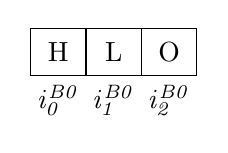
\begin{tikzpicture}
                \path
                    node[letter, label=below:{\id{i}{B0}{0}}] {H}
                    to ++(0:\widthletter) node[letter, label=below:{\id{i}{B0}{1}}] {L}
                    to ++(0:\widthletter) node[letter, label=below:{\id{i}{B0}{2}}] {O};
            \end{tikzpicture}
            \label{fig:logootsplit-seq-as-letters}
        \end{minipage}}
    \hfil
    \subfloat[Elements grouped into a block]{
        \begin{minipage}{.48\linewidth}
        \centering
            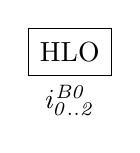
\begin{tikzpicture}
                \path
                    node[block, label=below:{\id{i}{B0}{0..2}}] {HLO};
            \end{tikzpicture}
            \label{fig:logootsplit-seq-as-block}
        \end{minipage}}
    \caption{Representation of a LogootSplit sequence containing the elements "HLO"}
    \label{fig:logootsplit-seq}
\end{figure}

This feature reduces the number of identifiers stored in the data structure, since identifiers are kept at the level of blocks rather than on every individual element.
It enables to reduce significantly the memory overhead of the data structure.

\subsection{Limits}

As stated previously, the size of identifiers from a dense total order is variable.
When nodes insert new elements between two others with the same \emph{position} value, LogootSplit has no other option but to increase the size of the resulting identifiers.
\autoref{fig:example-split} illustrates such cases.
In this example, since node A inserts a new element between the contiguous identifiers \id{i}{B0}{0} and \id{i}{B0}{1}, LogootSplit can not generate a proper identifier of the same size.
To comply with the intended order, LogootSplit generates a new identifier by appending a new tuple to the identifier of the predecessor : \id{i}{B0}{0}\id{f}{A0}{0}.

\begin{figure}[h!]
    \centering
    \begin{tikzpicture}
        \path
            node {\textbf{A}}
            to ++(0:\widthletter) node[block, label=below:{\id{i}{B0}{0..2}}] (HLO) {HLO}
            to ++(0:5 * \widthletter) node[letter, label=below:{\id{i}{B0}{0}}] (H) {H}
            to ++(0:\widthletter) node[letter, fill=mydarkorange, label=above:{\color{mydarkorange}\id{i}{B0}{0}\id{f}{A0}{0}}] {E}
            to ++(0:\widthletter) node[block, label=below:{\id{i}{B0}{1..2}}] {LO};

        \draw[->, thick] (HLO) -- node[below, align=center]{\emph{insert "e"}\\\emph{between}\\\emph{"h" and "l"}} (H);
    \end{tikzpicture}
    \caption{Insertion leading to longer identifiers}
    \label{fig:example-split}
\end{figure}

As a result, the size of identifiers tends to grow as the system progresses.
This growth impacts negatively the performance of the data structure on several aspects.
Since identifiers attached to values become longer, the memory overhead of the data structure increases accordingly.
This also increases the bandwidth consumption as nodes have to broadcast identifiers to others.

Additionally, during the lifetime of the replicated sequence, the number of blocks increases.
Indeed, several constraints on identifier generation prevent nodes from adding new elements to existing blocks.
For example, only the node that generated the block can append or prepend elements to it.
These limitations cause the generation of new blocks.
The sequence ends up fragmented into many blocks of only few characters each.
However no mechanism to merge blocks a posteriori is provided.
The efficiency of the data structure hence decreases as each block introduces its own overhead.

As shown later in \autoref{sec:evaluation}, we measured that content eventually represents less than 1\% of the whole data structure size.
Remaining 99\% of the data structure hence correspond to metadata.
It is thus necessary to address the previously highlighted issues.

\section{Overview}
\label{sec:overview}

We propose a new Sequence \ac{CRDT} belonging to the variable-size identifiers approach: RenamableLogootSplit \cite{nicolas:hal-01932552,nicolas:hal-02526724}.
This data structure allows nodes to insert or remove elements into a replicated sequence.
We introduce a \emph{rename} operation to reassign shorter identifiers to elements and to group them into blocks to minimise the memory overhead of the whole sequence.

\subsection{System Model}

The system is composed of a dynamic set of nodes, as nodes join and leave dynamically the collaboration during its lifetime.
Nodes collaborate to build and maintain a sequence using RenamableLogootSplit.
Each node owns a copy of the sequence and edits it without any coordination.
Nodes' updates take the form of operations that are immediately applied to nodes' replicas.
Operations are then broadcast asynchronously to other nodes so that they also integrate updates.

Nodes communicate through a \ac{P2P} network, which is unreliable.
Messages can be lost, re-ordered or delivered multiple times.
The network is also vulnerable to partitions, which split nodes into disjoined subgroups.
To overcome failures of the network, nodes rely on a message-passing layer.
As RenamableLogootSplit is built on top of LogootSplit, it shares the same requirements for the operation delivery.
This layer is thus used to deliver messages to the application exactly-once.
The layer also ensures that \emph{remove} operations are delivered after corresponding \emph{insert} operations.
\mnnote{TODO: Ajouter une petite phrase pour exprimer qu'on a pas d'autres contraintes sur la livraison des opérations}
Nodes use an anti-entropy mechanism \cite{10.1109/TSE.1983.236733} to synchronise in a pairwise manner, by detecting and re-exchanging lost operations.

\subsection{Definition of the \emph{rename} operation}

\label{sec:definition-rename-operation}

The purpose of the \emph{rename} operation is to reassign new identifiers to elements of the replicated sequence without altering its content.
Since identifiers are metadata used by the data structure solely for conflict resolution, users are unaware of their existence.
\emph{Rename} operations are thus system operations: they are issued and applied by nodes behind the scenes, without any user initiative.

In order to ensure the \ac{SEC} property of the replicated sequence, we define several safety properties that the \emph{rename} operation must respect.
These properties are mainly inspired by those presented in \cite{zawirski:hal-01248197}.

\begin{property}(Determinism)
    \emph{Rename} operations are applied by each node without any coordination.
    To ensure that each node reaches eventually the same state, a given \emph{rename} operation must always output the same new identifier from the current identifier.
\end{property}

\begin{property}(User-intention Preservation)
    Although the \emph{rename} operations itself has no user intention attached, it must not conflict with users actions.
    Notably, \emph{rename} operations must not cancel or alter the outcome, from users' points of view, of \emph{insert} and \emph{remove} operations.
\end{property}

\begin{property}(Well-formed Sequence)
    The replicated sequence must be well-formed.
    Applying a \emph{rename} operation to a well-formed sequence must then output a well-formed sequence.
    A well-formed sequence ensures the following properties:
    \begin{itemize}[noitemsep]
        \item[~]
        \begin{subproperty}(Unicity Preservation)
            Each identifier must be unique.
            Thus, for a given \emph{rename} operation, each identifier should be mapped to a distinct new identifier.
        \end{subproperty}
        \item[~]
        \begin{subproperty}(Order Preservation)
            The elements of the sequence must be sorted according to their identifiers.
            Therefore, the existing order between initial identifiers must be preserved by the \emph{rename} operation.
        \end{subproperty}
    \end{itemize}
\end{property}

\begin{property}(Commutativity with Concurrent Operations)
    \label{prop:commutativity}
    Concurrent operations may be delivered in different orders to each node.
    To ensure convergence of replicas, the order of application of a set of concurrent operations should not have any impact on the resulting state.
    The \emph{rename} operation must then be commutative with any other concurrent operation.
\end{property}

\autoref{prop:commutativity} is particularly difficult to achieve.
This is due to the fact that \emph{rename} operations modify identifiers assigned to elements.
However, other operations such as \emph{insert} and \emph{remove} ones rely on these identifiers to specify where to insert elements or which ones to remove.
\emph{Rename} operations are thus intrinsically incompatible with concurrent \emph{insert} and \emph{remove} ones.
Likewise, concurrent \emph{rename} operations may reassign different identifiers to given elements.
Concurrent \emph{rename} operations are hence not commutative.
Therefore, it is required to design and use conflict resolution strategies to achieve \autoref{prop:commutativity}.

For the sake of simplicity, the presentation of the \emph{rename} operation is divided into two parts.
In \autoref{sec:centralised-rls}, we present the proposed \emph{rename} operation under the assumption that no concurrent \emph{rename} operations may be issued.
This assumption enables us to focus on the inner working of the \emph{rename} operation and on how to deal with concurrent \emph{insert} and \emph{remove} operations.
Then, in \autoref{sec:distributed-rls}, we remove this assumption and present our approach to handle scenarios with concurrent \emph{rename} operations.

\section{RenamableLogootSplit without concurrent \emph{rename} operations}
\label{sec:centralised-rls}

\subsection{Proposed \emph{rename} operation}

\label{sec:rename-op}

Our \emph{rename} operation enables RenamableLogootSplit to reduce the overhead of nodes replica.
To do so, it reassigns arbitrary identifiers to elements.
Its behaviour is illustrated in \autoref{fig:renaming}.

\begin{figure}[h!]
    \centering
    \subfloat[Selecting the new identifier of the first element]{
        \begin{minipage}{\linewidth}
            \centering
            \begin{tikzpicture}
                \path
                    node {\textbf{A}}
                    to ++(0:\widthletter) node[letter, label=below:{\id{i}{B0}{0}}] {H}
                    to ++(0:\widthletter) node[letter, fill=mydarkorange, label=above:{\color{mydarkorange}\id{i}{B0}{0}\id{f}{A0}{0}}] {E}
                    to ++(0:\widthletter) node[block, label=below:{\id{i}{B0}{1..2}}] (LO) {LO}
                    to ++(0:4 * \widthletter) node[letter, fill=mydarkblue, label=below:{\color{mydarkblueid}\id{i}{A1}{0}}] (H) {H};

                \draw[->, thick] (LO) -- node[below, align=center]{\emph{rename}} (H);
            \end{tikzpicture}
            \label{fig:renaming-first-id}
        \end{minipage}}
    \hfil
    \subfloat[Selecting the new identifiers of the remaining ones]{
        \begin{minipage}{\linewidth}
            \centering
            \begin{tikzpicture}
                \path
                    node {\textbf{A}}
                    to ++(0:\widthletter) node[letter, label=below:{\id{i}{B0}{0}}] {H}
                    to ++(0:\widthletter) node[letter, fill=mydarkorange, label=above:{\color{mydarkorange}\id{i}{B0}{0}\id{f}{A0}{0}}] {E}
                    to ++(0:\widthletter) node[block, label=below:{\id{i}{B0}{1..2}}] (LO) {LO}
                    to ++(0:4 * \widthletter) node[letter, fill=mydarkblue, label=below:{\color{mydarkblueid}\id{i}{A1}{0}}] (H) {H}
                    to ++(0:\widthletter) node[letter, fill=mydarkblue, label=below:{\color{mydarkblueid}\id{i}{A1}{1}}] {E}
                    to ++(0:\widthletter) node[letter, fill=mydarkblue, label=below:{\color{mydarkblueid}\id{i}{A1}{2}}] {L}
                    to ++(0:\widthletter) node[letter, fill=mydarkblue, label=below:{\color{mydarkblueid}\id{i}{A1}{3}}] {O};

                    \draw[->, thick] (LO) -- node[below, align=center]{\emph{rename}} (H);
                \end{tikzpicture}
            \label{fig:renaming-second-id}
        \end{minipage}}
    \hfil
    \subfloat[Final state obtained]{
        \begin{minipage}{\linewidth}
            \centering
            \begin{tikzpicture}
                \path
                    node {\textbf{A}}
                    to ++(0:\widthletter) node[letter, label=below:{\id{i}{B0}{0}}] {H}
                    to ++(0:\widthletter) node[letter, fill=mydarkorange, label=above:{\color{mydarkorange}\id{i}{B0}{0}\id{f}{A0}{0}}] {E}
                    to ++(0:\widthletter) node[block, label=below:{\id{i}{B0}{1..2}}] (LO) {LO}
                    to ++(0:4 * \widthletter) node[block, fill=mydarkblue, label=below:{\color{mydarkblueid}\id{i}{A1}{0..3}}] (HELO) {HELO};

                \draw[->, thick] (LO) -- node[below, align=center]{\emph{rename}} (HELO);
            \end{tikzpicture}
            \label{fig:renaming-final-state}
        \end{minipage}}
    \caption{Renaming the sequence on node \emph{A}}
    \label{fig:renaming}
\end{figure}

In this example, node A initiates a \emph{rename} operation on its local state.
First, node A reuses the id of the first element of the sequence (\id{i}{B0}{0}) but modifies it with its own node id (\textbf{A}) and current sequence number (\emph{1}).
Also the offset is set to 0.
Node A reassigns the resulting id (\id{i}{A1}{0}) to the first element of the sequence as described in \autoref{fig:renaming-first-id}.
Then, node A derives contiguous identifiers for all remaining elements by successively incrementing the offset (\id{i}{A1}{1}, \id{i}{A1}{2} and \id{i}{A1}{3}), as shown in \autoref{fig:renaming-second-id}.
As we assign contiguous identifiers to all elements of the sequence, we eventually group them into one block as illustrated in \autoref{fig:renaming-final-state}.
It allows nodes to benefit the most from the block feature and to minimise the overhead of the resulting state.

To converge, other nodes have to rename their state identically.
However, they can not simply replace their current state with the new renamed one.
Indeed, they may have performed concurrent updates on their states.
In order not to discard these updates, nodes have to process the \emph{rename} operation themselves.
To this end, the node issuing the \emph{rename} operation broadcasts its \emph{former state} to others.
Using this state, other nodes compute the new identifier of each renamed identifier.
As for concurrently inserted identifiers, we explain in \autoref{sec:dealing-with-concurrent-updates} how nodes rename them in a deterministic way.

\subsection{Dealing with concurrent updates}

\label{sec:dealing-with-concurrent-updates}

% Before:
% As \emph{rename} operations can be issued without any kind of coordination, it is possible for other nodes to perform updates concurrently.
After applying \emph{rename} operations on their local state, nodes may receive concurrent updates.
Figure \ref{fig:concurrent-insert-rename-inconsistent} illustrates such cases.
In this example node B inserts the new element "L", assigns the id \id{i}{B0}{0}\id{m}{B1}{0} to it and broadcasts its update, concurrently to the \emph{rename} operation described in \autoref{fig:renaming}.
Upon reception of the \emph{insert} operation, node A adds the inserted element into its sequence, using the element id to determine its position.
However, since identifiers were modified by the concurrent \emph{rename} operation, node A inserts the new element at the end of its sequence (since \id{i}{A1}{3} < \id{i}{B0}{0}\id{m}{B1}{0}) instead of at the intended position.
As described by this example, applying naively concurrent updates would result in inconsistencies.
It is thus necessary to handle concurrent operations to \emph{rename} operations in a particular manner.

\begin{figure*}[h!]
    \centering
    \begin{tikzpicture}
        \path
            node {\textbf{A}}
            to ++(0:\widthletter) node[letter, label=below:{\id{i}{B0}{0}}] {H}
            to ++(0:\widthletter) node[letter, fill=mydarkorange, label=above:{\color{mydarkorange}\id{i}{B0}{0}\id{f}{\,A0}{0}}] {E}
            to ++(0:\widthletter) node[block, label=below:{\id{i}{B0}{1..2}}] (S0A-right) {LO}
            to ++(0:5 * \widthletter) node[block, fill=mydarkblue,
                    label={below:{\color{mydarkblueid}\id{i}{A1}{0..3}} }
                        ] (S1A) {HELO}
            to ++(0:8 * \widthletter) node[block, fill=mydarkblue,
                    label={below:{\color{mydarkblueid}\id{i}{A1}{0..3}} }
                        ] (S2A-left) {HELO}
            to ++(0:1.18 * \widthblock) node[letter, fill=mylightorange, cross,
                    label={above:{\color{mylightorange}\id{i}{B0}{0}\id{m}{B1}{0}} }
                        ] {L};

        \path
            to ++(270:2) node {\textbf{B}}
            to ++(0:\widthletter) node[letter, label=below:{\id{i}{B0}{0}}] {H}
            to ++(0:\widthletter) node[letter, fill=mydarkorange, label=above:{\color{mydarkorange}\id{i}{B0}{0}\id{f}{\,A0}{0}}] {E}
            to ++(0:\widthletter) node[block, label=below:{\id{i}{B0}{1..2}}] (S0B-right) {LO}
            to ++(0:5 * \widthletter) node[letter, label=below:{\id{i}{B0}{0}}] (S1B-left) {H}
            to ++(0:\widthletter) node[letter, fill=mydarkorange, label=above:{\color{mydarkorange}\id{i}{B0}{0}\id{f}{\,A0}{0}}] {E}
            to ++(0:\widthletter) node[letter, fill=mylightorange, label=below:{\color{mylightorange}\id{i}{B0}{0}\id{m}{B1}{0}}] {L}
            to ++(0:\widthletter) node[block, label=above:{\id{i}{B0}{1..2}}] (S1B-right) {LO};


        \draw[->, thick] (S0A-right) -- node[above, align=center]{\emph{rename}} (S1A);
        \draw[dotted] (S1A) -- (S2A-left);
        \draw[->, thick] (S0B-right) -- node[below, align=center]{\emph{insert "l"}\\\emph{between}\\\emph{"e" and "l"}} (S1B-left);
        \draw[dashed, ->, thick, shorten >= 3] (S1B-right.east) -- node[below right, align=center]{\emph{insert "l" at} {\color{mylightorange}\id{i}{B0}{0}\id{m}{B1}{0}}} (S2A-left.west);

    \end{tikzpicture}
    \caption{Concurrent update leading to inconsistency}
    \label{fig:concurrent-insert-rename-inconsistent}
\end{figure*}

First, nodes have to detect concurrent operations to \emph{rename} ones.
To this end, we use an \emph{epoch-based} system.
Initally, the replicated sequence starts at the \emph{origin} epoch noted \epoch{0}.
Each \emph{rename} operation introduces a new epoch and enables nodes to advance their states to it from the previous epoch.
The generated epoch is characterised using the node id and its current sequence number upon the generation of the \emph{rename} operation.
For example, the \emph{rename} operation described in \autoref{fig:concurrent-insert-rename-inconsistent} enables nodes to advance their states from \epoch{0} to \epoch{A1}.

As they receive \emph{rename} operations, nodes build and maintain the \emph{epoch chain}, a data structure ordering epochs according to their \emph{parent-child} relation.
Additionally, nodes tag every operation with their current epoch at the time the operation is generated.
Upon the reception of an operation, nodes compare the operation epoch to their current one.
If they differ, nodes have to transform the operation before applying it.
Nodes determine against which \emph{rename} operations to transform the received operation by computing the path between the operation epoch and their current one using the \emph{epoch chain}.
For this purpose, it is required to add the following rule to existing constraints upon the delivery of operations: operations must now be delivered after the \emph{rename} operation which introduced their epoch.

Nodes use the function $\trm{renameId}$, described in \autoref{alg:renameId}, to transform \emph{insert} or \emph{remove} operations against \emph{rename} ones.
% Before:
% Upon the reception of an operation, nodes compare the operation epoch to their current one.
% The main idea of this algorithm is to use the predecessor of the given identifier to do so.
This algorithm maps identifiers from a \emph{parent} epoch to corresponding ones in the \emph{child} epoch.
The main idea of this algorithm is to rename unknown identifiers at the time of the \emph{rename} operation generation using their predecessor.
An example of its usage is illustrated in \autoref{fig:concurrent-insert-rename-fixed}.
This figure depicts the same scenario as in \autoref{fig:concurrent-insert-rename-inconsistent}, except that this time node A uses \autoref{alg:renameId} to rename the concurrently generated id before inserting it in its state.

The algorithm proceeds as follows.
First, node A retrieves the predecessor of the given id \id{i}{B0}{0}\id{m}{B1}{0} in the former state: \id{i}{B0}{0}\id{f}{A0}{0}.
Then it computes the counterpart of \id{i}{B0}{0}\id{f}{A0}{0} in the renamed state: \id{i}{A1}{1}.
Finally, node A prepends it to the given id to generate the renamed id: \id{i}{A1}{1}\id{i}{B0}{0}\id{m}{B1}{0}.
By reassigning this id to the concurrently added element, node A is able to insert it in its state while preserving the intended order.

\begin{myalgorithm}[h!]
    \begin{algorithmic}
        \Function {renameId}{id, renamedIds, nId, nSeq}
            \State length $\gets$ renamedIds.length
            \State firstId $\gets$ renamedIds[0]
            \State lastId $\gets$ renamedIds[length - 1]
            \State pos $\gets$ position(firstId)
            \\
            \If{id < firstId}
                \State newFirstId $\gets$ \new~Id(pos, nId, nSeq, 0)
                \State \Return renIdLessThanFirstId(id, newFirstId)
            \ElsIf{id $\in$ renameIds}
                \State index $\gets$ findIndex(id, renamedIds)
                \State \Return \new~Id(pos, nId, nSeq, index)
            \ElsIf{lastId < id}
                \State newLastId $\gets$ \new~Id(pos, nId, nSeq, length - 1)
                \State \Return renIdGreaterThanLastId(id, newLastId)
            \Else
                \State \Return renIdFromPredId(id, renamedIds, pos, nId, nSeq)
            \EndIf
        \EndFunction
        \\
        \Function {renIdFromPredId}{id, renamedIds, pos, nId, nSeq}
            \State index $\gets$ findIndexOfPred(id, renamedIds)
            \State newPredId $\gets$ \new~Id(pos, nId, nSeq, index)
            \\
            \State \Return concat(newPredId, id)
        \EndFunction
    \end{algorithmic}
    \caption{Rename concurrently generated identifier}
    \label{alg:renameId}
\end{myalgorithm}

\begin{figure*}[h!]
    \centering
    \begin{tikzpicture}
        \path
            node {\textbf{A}}
            to ++(0:0.5 * \widthletter) node[epoch] {\epoch{0}}
            to ++(0:1.05 * \widthoriginepoch) node[letter, label=below:{\id{i}{B0}{0}}] {H}
            to ++(0:\widthletter) node[letter, fill=mydarkorange, label=above:{\color{mydarkorange}\id{i}{B0}{0}\id{f}{\,A0}{0}}] {E}
            to ++(0:\widthletter) node[block, label=below:{\id{i}{B0}{1..2}}] (S0A-right) {LO}
            to ++(0:5 * \widthletter) node[epoch] (S1A-left) {\epoch{A1}}
            to ++(0:1.3 * \widthepoch) node[block, fill=mydarkblue,
                    label={below:{\color{mydarkblueid}\id{i}{A1}{0..3}} }
                        ] (S1A-right) {HELO}
            to ++(0:8 * \widthletter) node[epoch] (S2A-left) {\epoch{A1}}
            to ++(0:1.3 * \widthepoch) node[block, fill=mydarkblue,
                    label={below:{\color{mydarkblueid}\id{i}{A1}{0..1}} }
                        ] {HE}
            to ++(0:\widthblock) node[letter, fill=mylightblue,
                    label={above:{\color{mylightblue!20!mydarkblueid}\id{i}{A1}{1}\id{i}{B0}{0}\id{m}{B1}{0}} }
                        ] {L}
            to ++(0:\widthletter) node[block, fill=mydarkblue,
                    label={below:{\color{mydarkblueid}\id{i}{A1}{2..3}} }
                        ] {LO};

        \path
            to ++(270:2) node {\textbf{B}}
            to ++(0:0.5 * \widthletter) node[epoch] {\epoch{0}}
            to ++(0:1.05 * \widthoriginepoch) node[letter, label=below:{\id{i}{B0}{0}}] {H}
            to ++(0:\widthletter) node[letter, fill=mydarkorange, label=above:{\color{mydarkorange}\id{i}{B0}{0}\id{f}{\,A0}{0}}] {E}
            to ++(0:\widthletter) node[block, label=below:{\id{i}{B0}{1..2}}] (S0B-right) {LO}
            to ++(0:5 * \widthletter) node[epoch] (S1B-left) {\epoch{0}}
            to ++(0:1.05 * \widthoriginepoch) node[letter, label=below:{\id{i}{B0}{0}}] {H}
            to ++(0:\widthletter) node[letter, fill=mydarkorange, label=above:{\color{mydarkorange}\id{i}{B0}{0}\id{f}{\,A0}{0}}] {E}
            to ++(0:\widthletter) node[letter, fill=mylightorange, label=below:{\color{mylightorange}\id{i}{B0}{0}\id{m}{B1}{0}}] {L}
            to ++(0:\widthletter) node[block, label=above:{\id{i}{B0}{1..2}}] (S1B-right) {LO};


        \draw[->, thick] (S0A-right) -- node[above, align=center]{\emph{rename to \epoch{A1}}} (S1A-left);
        \draw[dotted] (S1A-right) -- (S2A-left);
        \draw[->, thick] (S0B-right) -- node[below, align=center]{\emph{insert "l"}\\\emph{between}\\\emph{"e" and "l"}} (S1B-left);
        \draw[dashed, ->, thick, shorten >= 3] (S1B-right.east) -- node[below right, align=center]{\emph{insert "l" at} {\color{mylightorange}\id{i}{B0}{0}\id{m}{B1}{0}}} (S2A-left.west);

    \end{tikzpicture}
    \caption{Renaming concurrent update using \autoref{alg:renameId} before applying it to maintain intended order}
    \label{fig:concurrent-insert-rename-fixed}
\end{figure*}

% Before:
% As explained in \autoref{sec:rename-op}, some nodes may have applied concurrent \emph{insert} operations to their state before receiving a given remote \emph{rename} operation.
% \autoref{alg:renameId} also solves this case.
% It allows them to converge with nodes which processed the \emph{rename} operations before the concurrent \emph{insert} operations.
\autoref{alg:renameId} also enables nodes to handle the opposite case : to integrate remote \emph{rename} operations on their local state while they have previously applied concurrent updates.
This case corresponds to node B's one in \autoref{fig:concurrent-insert-rename-fixed}.
Upon the delivery of node A's \emph{rename} operation, applying \autoref{alg:renameId} to every identifiers of its state would enable node B to reach an equivalent state to node A's one.

\autoref{alg:renameId} features only the main case of $\trm{renameId}$, \ie when the identifier to rename is in the range of renamed identifiers ($\trm{firstId} \leq \trm{id} \leq \trm{lastId}$).
Functions to deal with other cases, \ie when the identifier to rename is out of the range of renamed identifiers ($\trm{id} < \trm{firstId}$ or $\trm{lastId} < \trm{id}$), are presented in \refappendix{app:rename-id}.

\subsection{Optimisations}

\label{sec:optimisations}

\mnnote{TODO: Ajouter une phrase ou deux pour introduire cette sous-section}

\headerparagraph{Garbage collection and offloading of former states}
%
Since nodes rely on the former state to transform concurrent operations to a \emph{rename} one, they have to store it.
Nodes need it until each of them can no longer issue concurrent operations to the corresponding \emph{rename} operation.
In other words, nodes can safely garbage collect the former state once the \emph{rename} operation became causally stable \cite{10.1007/978-3-662-43352-2_11}.
To determine that a given \emph{rename} operation is causally stable, nodes have to be aware of others and of their progress.
A group membership protocol such as \cite{swim2002,lifeguard2018} is thus required.

Causal stability may take some time to be achieved.
Meanwhile, nodes can actually offload former states onto the disk since they are only required to handle concurrent operations to \emph{rename} ones.
We discuss this topic further in \autoref{sec:offloading-former-states}.

\headerparagraph{Compression technique for \emph{rename} operations}
%
To limit bandwidth consumption of \emph{rename} operations, we propose the following compression technique.
Node may broadcast only necessary components to uniquely identify blocks instead of whole identifiers.
Indeed, an identifier can be uniquely identified from the \emph{node identifier}, \emph{node sequence number} and \emph{offset} of its last tuple.
A block can therefore be uniquely identified from these components and its length.
This reduces the data to send to a fixed amount per block.
To decompress the received operation, nodes browse their current state and log of concurrent \emph{remove} operations.
This allows them to retrieve whole identifiers and to reconstruct the original \emph{rename} operation.
Additionally, we can set an upper-bound to the size of \emph{rename} operations by issuing them as soon as the state reaches a given number of blocks.

\mnnote{QUESTION:
    Ajouter un paragraphe sur une version améliorée de \emph{renameId()} permettant de renommer par bloc plutôt que par id ?
    Permettrait de réduire sa complexité.
}

\section{RenamableLogootSplit with concurrent \emph{rename} operations}

\label{sec:distributed-rls}

\subsection{Concurrent \emph{rename} operations}

We now consider scenarios with concurrent \emph{rename} operations.
\autoref{fig:conflicting-rename-operations} expands the scenario previously described in \autoref{fig:concurrent-insert-rename-fixed} to depicts such one.

\begin{figure*}[h!]
    \centering
    \begin{tikzpicture}
        \path
            node {\textbf{A}}
            to ++(0:0.5 * \widthletter) node[epoch] {\epoch{0}}
            to ++(0:1.05 * \widthoriginepoch) node[letter, label=below:{\id{i}{B0}{0}}] {H}
            to ++(0:\widthletter) node[letter, fill=mydarkorange, label=above:{\color{mydarkorange}\id{i}{B0}{0}\id{f}{\,A0}{0}}] {E}
            to ++(0:\widthletter) node[block, label=below:{\id{i}{B0}{1..2}}] (S0A-right) {LO}
            to ++(0:5 * \widthletter) node[epoch] (S1A-left) {\epoch{A1}}
            to ++(0:1.3 * \widthepoch) node[block, fill=mydarkblue,
                    label={below:{\color{mydarkblueid}\id{i}{A1}{0..3}} }
                        ] (S1A-right) {HELO}
            to ++(0:8 * \widthletter) node[epoch] (S2A-left) {\epoch{A1}}
            to ++(0:1.3 * \widthepoch) node[block, fill=mydarkblue,
                    label={below:{\color{mydarkblueid}\id{i}{A1}{0..1}} }
                        ] {HE}
            to ++(0:\widthblock) node[letter, fill=mylightblue,
                    label={above:{\color{mylightblue!20!mydarkblueid}\id{i}{A1}{1}\id{i}{B0}{0}\id{m}{B1}{0}} }
                        ] {L}
            to ++(0:\widthletter) node[block, fill=mydarkblue,
                    label={below:{\color{mydarkblueid}\id{i}{A1}{2..3}} }
                        ] (S2A-right) {LO};
            % to ++(0:2) node (A-sync) {}
            % to ++(90:1) node (sync-top-left) {};

        \path
            to ++(270:3) node {\textbf{B}}
            to ++(0:0.5 * \widthletter) node[epoch] {\epoch{0}}
            to ++(0:1.05 * \widthoriginepoch) node[letter, label=below:{\id{i}{B0}{0}}] {H}
            to ++(0:\widthletter) node[letter, fill=mydarkorange, label=above:{\color{mydarkorange}\id{i}{B0}{0}\id{f}{\,A0}{0}}] {E}
            to ++(0:\widthletter) node[block, label=below:{\id{i}{B0}{1..2}}] (S0B-right) {LO}
            to ++(0:5 * \widthletter) node[epoch] (S1B-left) {\epoch{0}}
            to ++(0:1.05 * \widthoriginepoch) node[letter, label=below:{\id{i}{B0}{0}}] {H}
            to ++(0:\widthletter) node[letter, fill=mydarkorange, label=above:{\color{mydarkorange}\id{i}{B0}{0}\id{f}{\,A0}{0}}] {E}
            to ++(0:\widthletter) node[letter, fill=mylightorange, label=below:{\color{mylightorange}\id{i}{B0}{0}\id{m}{B1}{0}}] {L}
            to ++(0:\widthletter) node[block, label=above:{\id{i}{B0}{1..2}}] (S1B-right) {LO}
            to ++(0:5 * \widthletter) node[epoch] (S2B-left) {\epoch{B2}}
            to ++(0:1.3 * \widthepoch) node[block, fill=mydarkpurple,
                    label={ [] below:{\color{mydarkpurpleid}\id{i}{B2}{0..4}} }
                ] (S2B-right) {HELLO};
            % to ++(0:3.8) node (B-sync) {}
            % to ++(0:1.2)
            % to ++(270:1) node (sync-bottom-right) {};

        % \draw[thick] (sync-top-left) rectangle (sync-bottom-right) node [midway] (midway) {};

        % \path
        %     (midway)
        %     to ++(90:0.6) node {S}
        %     to ++(270:0.4) node {Y}
        %     to ++(270:0.4) node {N}
        %     to ++(270:0.4) node {C};

        \draw[->, thick] (S0A-right) -- node[above, align=center]{\emph{rename to \epoch{A1}}} (S1A-left);
        \draw[dotted] (S1A-right) -- (S2A-left); % (S2A-right) -- (A-sync) (S2B-right) -- (B-sync);
        \draw[->, thick] (S0B-right) -- node[below, align=center]{\emph{insert "l"}\\\emph{between}\\\emph{"e" and "l"}} (S1B-left);
        \draw[dashed, ->, thick, shorten >= 3] (S1B-right.east) -- node[right, xshift=5pt, align=center]{\emph{insert "l" at} {\color{mylightorange}\id{i}{B0}{0}\id{m}{B1}{0}}} (S2A-left.west);
        \draw[->, thick] (S1B-right) -- node[below, align=center]{\emph{rename to \epoch{B2}}} (S2B-left);


    \end{tikzpicture}
    \caption{Concurrent \emph{rename} operations leading to divergent states}
    \label{fig:conflicting-rename-operations}
\end{figure*}

After broadcasting its \emph{insert} operation, node B performs a \emph{rename} operation on its state.
This operation reassigns new identifiers to every element based on the id of the first element of the sequence (\id{i}{B0}{0}), its node id (\textbf{B}) and current sequence number (\emph{2}).
This operation also introduces a new epoch: \epoch{B2}.
Since node A's \emph{rename} operation was not yet delivered to node B at that moment, both \emph{rename} operations are concurrent.

% - Expliquer l'arbre des epochs
As concurrent epochs are generated, epochs now form the \emph{epoch tree}.
We represent in \autoref{fig:epoch-tree} the \emph{epoch tree} that nodes obtain once they eventually synchronise.
Epochs are displayed as nodes of the tree and the \emph{parent-child} relation between them displayed as black arrows.

\begin{figure}[h!]
    \centering
    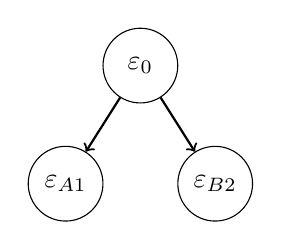
\begin{tikzpicture}
        \path
            node[op] (e0) {\epoch{0}}
            to ++(270:1.5)
            to ++(180:0.95) node[op] (eA1) {\epoch{A1}};
        \path
            to ++(270:1.5)
            to ++(0:0.95) node[op] (eB2) {\epoch{B2}};

        \draw[thick, ->] (e0) -- (eA1);
        \draw[thick, ->] (e0) -- (eB2);
    \end{tikzpicture}
    \caption{The \emph{epoch tree} corresponding to the scenario of \autoref{fig:conflicting-rename-operations}}
    \label{fig:epoch-tree}
\end{figure}

At the end of the scenario described in \autoref{fig:conflicting-rename-operations}, nodes A and B are respectively at epochs \epoch{A1} and \epoch{B2}.
In order to converge, every node should eventually reach the same epoch.
However, the function $\trm{renameId}$ described in \autoref{alg:renameId} only enables nodes to move from a \emph{parent} epoch to one of its \emph{children} epoch.
Nodes A and B are thus unable to progress towards the epoch of the other.
It is therefore necessary to extend our renaming mechanism to break this deadlock.

First, nodes have to agree on one epoch from the \emph{epoch tree} as the target epoch.
In order to avoid performance issues due to coordination, nodes should select this epoch in a coordination-free manner, \ie solely using data from the \emph{epoch tree}.
We propose such a mechanism in \autoref{sec:priority}.

Second, nodes have to move throught the \emph{epoch tree} to reach the target epoch.
The function $\trm{renameId}$ already enables nodes to move down the tree.
Remaining cases to be handled are the ones in which nodes are currently at \emph{sibling} or \emph{cousin} epochs of the target one.
In these cases, nodes have to be able to move up the \emph{epoch tree} to return to the \ac{LCA} of the current epoch and the target one.
This move is actually akin to reverting the effect of previously applied \emph{rename} operations.
We propose an algorithm that fulfills this purpose in \autoref{sec:reverting-rename-ops}.

\subsection{Breaking tie between concurrent \emph{rename} operations}
\label{sec:priority}

To enable every nodes to select in a coordination-free manner the same target epoch, we define \emph{priority}, a total order relation between epochs.

To define the \emph{priority} relation, we may actually select different strategies.
In this work, we use the lexicographical order on the path of epochs in the \emph{epoch tree}.
\autoref{fig:priority-example} provides an example of its use.

\begin{figure}[h!]
    \subfloat[Example of execution with concurrent \emph{rename} operations]{
        \begin{minipage}{\linewidth}
            \centering
            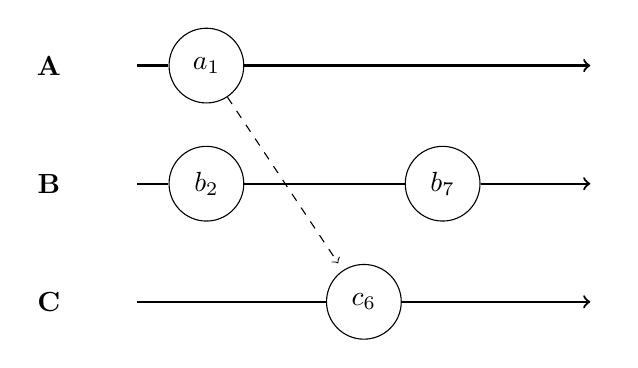
\begin{tikzpicture}
                \path
                    node {\textbf{A}}
                    to ++(0:1) node (a0) {}
                    to ++(0:1) node[op] (a1) {$a_1$}
                    to ++(0:5) node (a-end) {};

                \draw[->, thick] (a0) --  (a1) -- (a-end);

                \path
                    to ++(270:1.5) node {\textbf{B}}
                    to ++(0:1) node (b0) {}
                    to ++(0:1) node[op] (b2) {$b_2$}
                    to ++(0:3) node[op] (b7) {$b_7$}
                    to ++(0:2) node (b-end) {};

                \draw[->, thick] (b0) -- (b2) -- (b7) -- (b-end);

                \path
                    to ++(270:3) node {\textbf{C}}
                    to ++(0:1) node (c0) {}
                    to ++(0:3) node[op] (c6) {$c_6$}
                    to ++(0:3) node (c-end) {};

                \draw[->, thick] (c0) -- (c6) -- (c-end);

                \draw[->, dashed, shorten >= 3] (a1) -- (c6);
            \end{tikzpicture}
            \label{fig:priority-execution}
        \end{minipage}}
    \hfil
    \subfloat[Corresponding epoch tree with \emph{priority} relation shown]{
        \begin{minipage}{\linewidth}
            \centering
            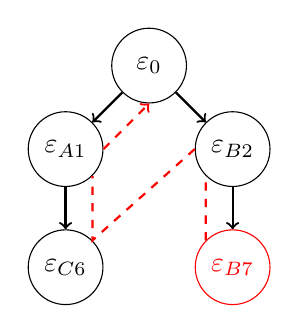
\begin{tikzpicture}
                \path
                    node[op] (e0) {\epoch{0}}
                    to ++(225:1.5) node[op] (eA1) {\epoch{A1}}
                    to ++(270:1.5) node[op] (eC6) {\epoch{C6}};
                \path
                    to ++(315:1.5) node[op] (eB2) {\epoch{B2}}
                    to ++(270:1.5) node[op, red] (eB7) {\epoch{B7}};

                \draw[->, thick] (e0) edge (eA1) (eA1) edge (eC6) (e0) edge (eB2) (eB2) edge (eB7);
                \draw[->, dashed, thick, red] (eB7.135) -- (eB2.225) (eB2.180) -- (eC6.45) -- (eA1.315) (eA1.0) -- (e0.270);
            \end{tikzpicture}
            \label{fig:priority-epoch-tree}
        \end{minipage}}
    \caption{Selecting target epoch from execution with concurrent \emph{rename} operations}
    \label{fig:priority-example}
\end{figure}

\autoref{fig:priority-execution} describes an execution in which the three nodes A, B and C issue several operations before eventually synchronising.
As solely \emph{rename} operations are relevant to the problem at hand, only them are represented in this figure.
Initially, node A issues a \emph{rename} operation introducing the epoch \epoch{A1}.
This operation is delivered to node C, which later issues its own \emph{rename} operation creating \epoch{C6}.
Concurrently to these operations, node B issues two \emph{rename} operations, generating \epoch{B2} then \epoch{B7}.

Once nodes synchronised, they obtain the \emph{epoch tree} represented in \autoref{fig:priority-epoch-tree}.
In this figure, the red dashed arrow represents the order between epochs according to the \emph{priority} relation while the selected target epoch is displayed as a red node.

To determine the target epoch, nodes rely on the \emph{priority} relation.
According to the lexicographical order on the path of epochs in the \emph{epoch tree}, \epoch{0} < \epoch{0}\epoch{A1} < \epoch{0}\epoch{A1}\epoch{C6} < \epoch{0}\epoch{B2} < \epoch{0}\epoch{B2}\epoch{B7}.
Therefore every node selects \epoch{B7} as the target epoch in a coordination-free manner.

Other strategies could be proposed to define the \emph{priority} relation.
For example, \emph{priority} could rely on metrics embedded in \emph{rename} operations representing the accumulated work on the document.
This topic will be further discussed in \autoref{sec:designing-more-effective-priority-relation}.

\subsection{Reverting \emph{rename} operations}

\label{sec:reverting-rename-ops}

We now introduce the function $\trm{revertRenameId}$.
Described in \autoref{alg:revertRenameId}, this function enables nodes to revert previously applied \emph{rename} operations.
To this end, $\trm{revertRenameId}$ maps identifiers from \emph{children} epoch to equivalent ones in their \emph{parent} epoch.

\begin{myalgorithm}[h!]
    \begin{algorithmic}
        \Function{revertRenameId}{id, renamedIds, nId, nSeq}
            % \Statex \LeftComment{$id}$ is the identifier to reverse rename}
            % \Statex \LeftComment{$renamedIds}$ is the former state shared by the \emph{rename} op}
            % \Statex \LeftComment{$nId}$ is $node~id}$ of the node which issued the \emph{rename} op}
            % \Statex \LeftComment{$nSeq}$ is $node~seq}$ of the node which issued the \emph{rename} op}
            % \\
            \State length $\gets$ renamedIds.length
            \State firstId $\gets$ renamedIds[0]
            \State lastId $\gets$ renamedIds[length - 1]
            \State pos $\gets$ getPosition(firstId)
            \\
            \State predOfNewFirstId $\gets$ \new~Id(pos, nId, nSeq, -1)
            \State newFirstId $\gets$ \new~Id(pos, nId, nSeq, 0)
            \State newLastId $\gets$ \new~Id(pos, nId, nSeq, length - 1)
            \\
            \If{id < newFirstId}
                \State \Return revRenIdLessThanNewFirstId(id, firstId, newFirstId)
            \ElsIf{isRenamedId(id, pos, nId, nSeq, length)}
                \State index $\gets$ getFirstOffset(id)
                \State \Return renamedIds[index]
            \ElsIf{newLastId < id}
                \State \Return revRenIdGreaterThanNewLastId(id, lastId)
            \Else
                % Ajouter commentaire sur cas
                \State index $\gets$ getFirstOffset(id)
                \State \Return revRenIdfromPredId(id, renamedIds, index)
            \EndIf
        \EndFunction
        \\
        \Function{revRenIdfromPredId}{id, renamedIds, index}
            \State predId $\gets$ renamedIds[index]
            \State succId $\gets$ renamedIds[index + 1]
            \State tail $\gets$ getTail(id, 1)
            \\
            \If{tail < predId}
                \State \Return concat(predId, MIN\_TUPLE, tail)
            \ElsIf{succId < tail}
                \State offset $\gets$ getLastOffset(succId) - 1
                \State predOfSuccId $\gets$ createIdFromBase(succId, offset)
                \State \Return concat(predOfSuccId, MAX\_TUPLE, tail)
            \Else
                \State \Return tail
            \EndIf
        \EndFunction
    \end{algorithmic}
    \caption{Revert rename identifier}
    \label{alg:revertRenameId}
\end{myalgorithm}

\mnnote{TODO: Ajouter commentaire dans l'algo pour préciser le cas où on rename un id inséré de façon concurrente ou causale au rename}

The goals of $\trm{revertRenameId}$ are the following:
\begin{enumerate*}[label=(\roman*)]
    \item To revert identifiers generated causally before or concurrently to the reverted \emph{rename} operation to their former value
    \item To assign new identifiers complying with the intended order to elements inserted causally after the reverted \emph{rename} operation.
\end{enumerate*}
We illustrate its behaviour with the help of \autoref{fig:revertRenameId}.

\begin{figure*}[h!]
    \centering
    \begin{tikzpicture}
        \path
            node {\textbf{A}}
            % to ++(0:0.5 * \widthletter) node (A-origin) {}
            % to ++(0:\widthletter) node (A-former) {}
            % to ++(0:3 * \widthletter) node[epoch] (S1A-left) {\epoch{A1}}
            to ++(0:0.5 * \widthletter) node[epoch] (S1A-left) {\epoch{A1}}
            to ++(0:1.3 * \widthepoch) node[block, fill=mydarkblue,
                    label={below:{\color{mydarkblueid}\id{i}{A1}{0..3}} }
                        ] (S1A-right) {HELO}
            to ++(0:8 * \widthletter) node[epoch] (S2A-left) {\epoch{A1}}
            to ++(0:1.3 * \widthepoch) node[block, fill=mydarkblue,
                    label={below:{\color{mydarkblueid}\id{i}{A1}{0..1}} }
                        ] {HE}
            to ++(0:\widthblock) node[letter, fill=mylightblue,
                    label={above:{\color{mylightblue!20!mydarkblueid}\id{i}{A1}{1}\id{i}{B0}{0}\id{m}{B1}{0}} }
                        ] {L}
            to ++(0:\widthletter) node[block, fill=mydarkblue,
                    label={below:{\color{mydarkblueid}\id{i}{A1}{2..3}} }
                        ] (S2A-right) {LO}
            to ++(0:2 * \widthblock) node (between-S2A-S3A) {}
            to ++(0:3 * \widthletter) node[epoch] (S3A-left) {\epoch{0}}
            to ++(0:1.05 * \widthoriginepoch) node[letter, label=below:{\id{i}{B0}{0}}] {H}
            to ++(0:\widthletter) node[letter, fill=mydarkorange, label=above:{\color{mydarkorange}\id{i}{B0}{0}\id{f}{\,A0}{0}}] {E}
            to ++(0:\widthletter) node[letter, fill=mylightorange, label=below:{\color{mylightorange}\id{i}{B0}{0}\id{m}{B1}{0}}] {L}
            to ++(0:\widthletter) node[block, label=above:{\id{i}{B0}{1..2}}] {LO};

        \path
            to ++(270:3) node {\textbf{B}}
            % to ++(0:0.5 * \widthletter) node (B-origin) {}
            % to ++(0:\widthletter) node (B-former) {}
            % to ++(0:3 * \widthletter) node[epoch] (S1B-left) {\epoch{0}}
            to ++(0:0.5 * \widthletter) node[epoch] (S1B-left) {\epoch{0}}
            to ++(0:1.05 * \widthoriginepoch) node[letter, label=below:{\id{i}{B0}{0}}] {H}
            to ++(0:\widthletter) node[letter, fill=mydarkorange, label=above:{\color{mydarkorange}\id{i}{B0}{0}\id{f}{\,A0}{0}}] {E}
            to ++(0:\widthletter) node[letter, fill=mylightorange, label=below:{\color{mylightorange}\id{i}{B0}{0}\id{m}{B1}{0}}] {L}
            to ++(0:\widthletter) node[block, label=above:{\id{i}{B0}{1..2}}] (S1B-right) {LO}
            to ++(0:5 * \widthletter) node[epoch] (S2B-left) {\epoch{B2}}
            to ++(0:1.3 * \widthepoch) node[block, fill=mydarkpurple,
                    label={ [] below:{\color{mydarkpurpleid}\id{i}{B2}{0..4}} }
                ] (S2B-right) {HELLO};

        % \draw[dotted] (A-origin) -- (A-former) (B-origin) -- (B-former);
        % \draw[->, thick] (A-former) -- node[above, align=center]{\emph{rename to \epoch{A1}}} (S1A-left);
        \draw[dotted] (S1A-right) -- (S2A-left);
        % \draw[->, thick] (B-former) -- node[below, align=center]{\emph{insert "l"}\\\emph{between}\\\emph{"e" and "l"}} (S1B-left);
        \draw[dashed, ->, thick, shorten >= 3] (S1B-right.east) -- node[right, xshift=5pt, align=center]{\emph{insert "l" at} {\color{mylightorange}\id{i}{B0}{0}\id{m}{B1}{0}}} (S2A-left.west);
        \draw[->, thick] (S1B-right) -- node[below, align=center]{\emph{rename to \epoch{B2}}} (S2B-left);
        \draw[dotted] (S2A-right) -- (between-S2A-S3A);
        \draw[dashed, thick] (S2B-right.east) -- node[right, xshift=5pt, align=center]{\emph{rename to \epoch{B2}}} (between-S2A-S3A);
        \draw[dashed, ->, thick] (between-S2A-S3A) -- node[above, align=center]{\emph{revert rename}\\\emph{to \epoch{A1}}} (S3A-left);
    \end{tikzpicture}
    \caption{Reverting a previously applied \emph{rename} operation}
    \label{fig:revertRenameId}
\end{figure*}

This figure resumes the scenario from \autoref{fig:conflicting-rename-operations}.
Node A is delivered node B's \emph{rename} operation, which is concurrent to A's one.
According to the proposed \emph{priority} relation, node A determines the introduced epoch \epoch{B2} as the target one.
It thus proceeds to revert its state to an equivalent one at \epoch{0}, the \ac{LCA} of its current epoch \epoch{A1} and the target one \epoch{B2}.
To this end, it applies $\trm{revertRenameId}$ to every identifiers of its current state.

$\trm{revertRenameId}$ determines which strategy to apply to revert the given identifier using patterns.
For example, identifiers of the form \id{pos}{nId~nSeq}{offset} (\id{i}{A1}{offset} in the current example) corresponds to the new values of the identifiers which were originally renamed.
To retrieve the original identifiers, $\trm{revertRenameId}$ simply uses their offset as it is their index in \emph{renamedIds}.

% According to its structure, \id{i}{A1}{1}\id{i}{B0}{0}\id{m}{B1}{0} may result from the transformation using $\trm{renIdFromPredId}$ of a identifier concurrently inserted to the \emph{rename} operation.
% Indeed, this identifier is composed of a prefix (\id{i}{A1}{1}) and a tail (\id{i}{B0}{0}\id{m}{B1}{0}), with the tail is between
% To revert the effect of the \emph{rename} operation, $\trm{revertRenameId}$ returns the tail.
% % To revert the effect of the \emph{rename} operation, $\trm{revertRenameId}$ first removes its prefix (\id{i}{A1}{1}) to isolate its tail (\id{i}{B0}{0}\id{m}{B1}{0}).
% The algorithm then compare the tail to the identifiers of its predecessor and successor at the \emph{parent} epoch.
% In this case, we have \id{i}{B0}{0}\id{f}{A0}{0} < \id{i}{B0}{0}\id{m}{B1}{0} < \id{i}{B0}{1}.
% $\trm{revertRenameId}$ can thus return the tail, as it

For other identifiers such as \id{i}{A1}{1}\id{i}{B0}{0}\id{m}{B1}{0}, \autoref{alg:revertRenameId} removes its prefix (\id{i}{A1}{1}) to isolate its tail (\id{i}{B0}{0}\id{m}{B1}{0}).
The algorithm then compare the tail to the identifiers of its predecessor and successor at the \emph{parent} epoch.
In this example, we have \id{i}{B0}{0}\id{f}{A0}{0} < \id{i}{B0}{0}\id{m}{B1}{0} < \id{i}{B0}{1}.
The algorithm can thus return the tail, as its value is between the identifiers of its predecessor and successor and preserve the intended order.
If it would not, \autoref{alg:revertRenameId} would use exclusive tuples of the renaming mechanism, $\trm{MIN\_TUPLE}$ and $\trm{MAX\_TUPLE}$, to generate an identifier complying with the intended order.

Once node A mapped its state to the equivalent one at \epoch{0} using \autoref{alg:revertRenameId}, it can now apply $\trm{renameId}$ to compute the corresponding state at \epoch{B2}.

As with \autoref{alg:renameId}, \autoref{alg:revertRenameId} only features the main case of $\trm{revertRenameId}$.
It corresponds to the case where the identifier to revert is in the range of renamed identifiers ($\trm{newFirstId} \leq \trm{id} \leq \trm{newLastId}$).
Functions to handle the rest of cases are featured in \refappendix{app:revert-rename-id}.

Note that $\trm{renameId}$ and $\trm{revertRenameId}$ are not inverse functions.
$\trm{revertRenameId}$ reverts to their original value identifiers inserted causally before or concurrently to the \emph{rename} operation.
But on the other hand, $\trm{renameId}$ does not do the same for identifiers inserted causally after the \emph{rename} operation.
Thus redoing a previously undone \emph{rename} operation alter these identifiers.
This alteration may cause a divergence between nodes, as the same element will be referred to using different identifiers.

This issue is however prevented in our system by the proposed \emph{priority} relation.
Since the \emph{priority} relation is defined using the lexicographical order on the path of epochs in the \emph{epoch tree}, nodes only move towards the rightmost epoch of the \emph{epoch tree} when switching epochs.
Nodes thus avoid going back and forth between different epochs and undoing then redoing corresponding \emph{rename} operations.

Nonetheless, the requirement to prevent nodes from redoing \emph{rename} operation limits our possibilities to design new \emph{priority} relations.
It would be interesting to remove this constraint to propose more effective \emph{priority} relations, as discussed in \autoref{sec:designing-more-effective-priority-relation}.
It can be achieved by designing a set of inverse functions for $\trm{renameId}$ and $\trm{revertRenameId}$.
Another solution is to propose an alternative implementation of the renaming mechanism that use the original identifiers instead of transformed ones, for example by relying on an \emph{operation log}.

\subsection{Garbage collection of \emph{former states}}

Nodes store epochs and corresponding \emph{former states} to map identifiers from previous or concurrent epochs to the current one.
However, once nodes become aware that some epochs can not possibly be required anymore to apply future operations, they can garbage collect these epochs and their corresponding \emph{rename} operations.
But, in systems which allow the generation of concurrent \emph{rename} operations, nodes can not solely rely on causal stability of \emph{rename} operations to determine which operations can be garbage collected.
Therefore, we propose the two following rules to enable nodes to identify unnecessary epochs:

\begin{myrule}
    \label{rule:gc-concurrent-primary-epoch}
    An epoch \epoch{} can be garbage collected if \epoch{} is a leaf of the epoch tree and a concurrent primary epoch \epoch{}' is causally stable.
\end{myrule}

\begin{myrule}
    \label{rule:gc-root}
    An epoch \epoch{} can be garbage collected if \epoch{} is the root of the epoch tree, has only one child \epoch{}' and that \epoch{}' is causally stable.
\end{myrule}

\autoref{fig:GC-epochs} illustrates a use case of \autoref{rule:gc-concurrent-primary-epoch} and \autoref{rule:gc-root}.
In \autoref{fig:GC-execution}, we represent an execution in which two nodes A and B respectively issue two \emph{rename} operation before eventually synchronising.
The operations shown in \autoref{fig:GC-execution} are solely \emph{rename} operations, as only these operations are relevant to the problem at hand.
In \autoref{fig:GC-epoch-trees-step-1}, we represent the states of their respective \emph{epoch trees} once they each generate their \emph{rename} operations.
In \autoref{fig:GC-epoch-trees-step-2}, we represent the new states of their \emph{epoch trees} once they each receive the first \emph{rename} operation issued by each other.
Epochs introduced by causally stable \emph{rename} operations are represented in \emph{epoch trees} using double circles.
The \emph{origin} epoch \epoch{0} is considered as causally stable from the beginning by design.
Epochs that are no longer necessary by applying \autoref{rule:gc-concurrent-primary-epoch} and \autoref{rule:gc-root} are respectively displayed as blue dashed nodes and green dotted nodes.

Upon the delivery of the \emph{rename} operation introducing epoch \epoch{B2} to node A, \epoch{B2} becomes causally stable.
From this point, node A knows that every node switched to this epoch at least.
Therefore nodes can no longer issue operations from \epoch{0}, \epoch{A1} or \epoch{A8}.
Thus these epochs and the \emph{rename} operations enabling nodes to switch between them can now be garbage collected.
\autoref{rule:gc-concurrent-primary-epoch} enables node A to garbage collect epochs \epoch{A8} then \epoch{A1}.
Then \autoref{rule:gc-root} enables node A to garbage collect \epoch{0} and the \emph{renaming} operation to switch to \epoch{B2}.

On the other hand, upon the reception of the \emph{rename} operation introducing \epoch{A1}, node B can not garbage collect any epochs despite \epoch{A1} being causally stable.
Indeed, from its point of view, other nodes may still issue operations from epoch \epoch{A1}.
Since in that case node B would have to transform operations to apply them to \epoch{B8}, node B has to retain all epochs forming the path between \epoch{A1} and \epoch{B8} and their corresponding \emph{rename} operations.

Eventually, once the system becomes idle, the current \emph{primary} epoch will become causally stable.
Nodes will then be able to garbage collect all other epochs using \autoref{rule:gc-concurrent-primary-epoch} and \autoref{rule:gc-root}, effectively suppressing the overhead of the renaming mechanism.

\begin{figure}[h!]
    \subfloat[Execution]{
        \begin{minipage}{\linewidth}
            \centering
            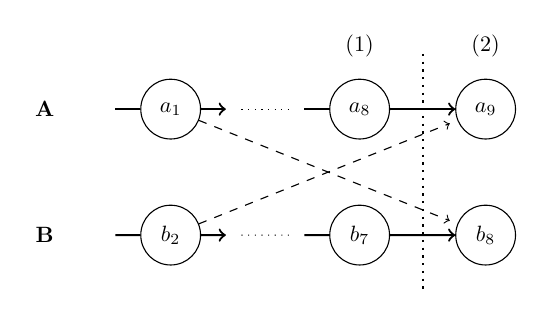
\begin{tikzpicture}[scale=0.8,every node/.style={scale=0.8}]
                \path
                    node {\textbf{A}}
                    to ++(0:1) node (a0) {}
                    to ++(0:1) node[op] (a1) {$a_1$}
                    to ++(0:1) node (a2) {}
                    to ++(0:1) node (a7) {}
                    to ++(0:1) node[op] (a8) {$a_8$}
                    to ++(90:1) node {(1)}
                    to ++(0:1) node (hideTop) {}
                    to ++(270:1)
                    to ++(0:1) node[op] (a9) {$a_9$}
                    to ++(90:1) node {(2)};

                \draw[->, thick] (a0) --  (a1) -- (a2);
                \draw[dotted] (a2) -- (a7);
                \draw[->, thick] (a7) -- (a8) -- (a9);

                \path
                    to ++(270:2) node {\textbf{B}}
                    to ++(0:1) node (b0) {}
                    to ++(0:1) node[op] (b2) {$b_2$}
                    to ++(0:1) node (b3) {}
                    to ++(0:1) node (b6) {}
                    to ++(0:1) node[op] (b7) {$b_7$}
                    to ++(0:1)
                    to ++(270:1) node (hideBot) {}
                    to ++(90:1)
                    to ++(0:1) node[op] (b8) {$b_8$};

                \draw[->, thick] (b0) -- (b2) -- (b3);
                \draw[dotted] (b3) -- (b6);
                \draw[->, thick] (b6) -- (b7) -- (b8);

                \draw[->, dashed, shorten >= 3] (a1) -- (b8);
                \draw[->, dashed, shorten >= 3] (b2) -- (a9);

                \draw[dotted, thick] (hideTop) -- (hideBot);
            \end{tikzpicture}
            \label{fig:GC-execution}
        \end{minipage}}
    \hfil
    \subfloat[States of respective epoch trees at (1)]{
        \begin{minipage}{\linewidth}
            \centering
            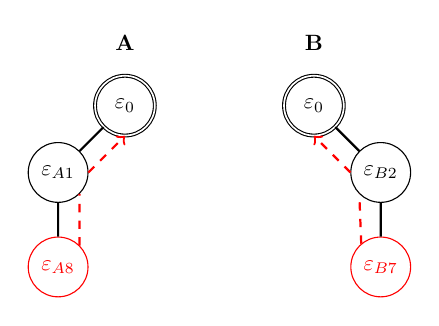
\begin{tikzpicture}[scale=0.8,every node/.style={scale=0.8}]
                \path
                    node {\textbf{A}}
                    to ++(270:1) node[causalop] (AeA0) {\epoch{0}}
                    to ++(225:1.5) node[op] (AeA1) {\epoch{A1}}
                    to ++(270:1.5) node[op, red] (AeA8) {\epoch{A8}};

                \path
                    to ++(0:3) node {\textbf{B}}
                    to ++(270:1) node[causalop] (BeB0) {\epoch{0}}
                    to ++(315:1.5) node[op] (BeB2) {\epoch{B2}}
                    to ++(270:1.5) node[op, red] (BeB7) {\epoch{B7}};


                \draw[thick] (AeA0) -- (AeA1) -- (AeA8);
                \draw[thick] (BeB0) -- (BeB2) -- (BeB7);
                \draw[->, dashed, thick, red] (AeA8.45) -- (AeA1.315) (AeA1.0) -- (AeA0.270);
                \draw[->, dashed, thick, red] (BeB7.130) -- (BeB2.225) (BeB2.180) -- (BeB0.270);

            \end{tikzpicture}
            \label{fig:GC-epoch-trees-step-1}
        \end{minipage}}
    \hfil
    \subfloat[States of respective epoch trees at (2)]{
        \begin{minipage}{\linewidth}
            \centering
            \begin{tikzpicture}[scale=0.8,every node/.style={scale=0.8}]
                \path
                    node {\textbf{A}}
                    to ++(270:1) node[op, gc-rule-2] (Ae0) {\epoch{0}}
                    to ++(225:1.5) node[op, gc-rule-1] (AeA1) {\epoch{A1}}
                    to ++(270:1.5) node[op, gc-rule-1] (AeA8) {\epoch{A8}};
                \path
                    to ++(270:1)
                    to ++(315:1.5) node[causalop] (AeB2) {\epoch{B2}}
                    to ++(270:1.5) node[op, red] (AeA9) {\epoch{A9}};

                \path
                    to ++(0:4) node {\textbf{B}}
                    to ++(270:1) node[causalop] (Be0) {\epoch{0}}
                    to ++(315:1.5) node[op] (BeB2) {\epoch{B2}}
                    to ++(270:1.5) node[op] (BeB7) {\epoch{B7}}
                    to ++(270:1.5) node[op, red] (BeB8) {\epoch{B8}};
                \path
                    to ++(0:4)
                    to ++(270:1)
                    to ++(225:1.5) node[causalop] (BeA1) {\epoch{A1}};


                \draw[thick] (Ae0) -- (AeA1) -- (AeA8) (Ae0) -- (AeB2) -- (AeA9);
                \draw[thick] (Be0) -- (BeB2) -- (BeB7) -- (BeB8) (Be0) -- (BeA1);
                \draw[->, dashed, thick, red] (AeA9.135) -- (AeB2.225) (AeB2.180) -- (AeA8.45) -- (AeA1.315) (AeA1.0) -- (Ae0.270);
                \draw[->, dashed, thick, red] (BeB8.135) -- (BeB7.225) (BeB7.135) -- (BeB2.225) (BeB2.180) -- (BeA1.0) -- (Be0.270);

            \end{tikzpicture}
            \label{fig:GC-epoch-trees-step-2}
        \end{minipage}}
    \caption{Garbage collecting epochs and corresponding \emph{former states}}
    \label{fig:GC-epochs}
\end{figure}

\section{Evaluation}

\label{sec:evaluation}

\subsection{Simulations and benchmarks}

In order to validate the proposed approach, we proceed to an experimental evaluation.
The aims of this evaluation are to measure
\begin{enumerate*}[label=(\roman*)]
    \item the memory overhead of the replicated sequence
    \item the computational overhead added to \emph{insert} and \emph{remove} operations by the renaming mechanism
    \item the cost of integrating \emph{rename} operations.
\end{enumerate*}

\mnnote{TODO: Reformuler paragraphe pour juste dire qu'on a utilisé des simulations pour notre évaluation (plutôt que d'insister sur le fait qu'on a pas réussi à avoir de traces réelles)}
% We proceed to evaluation by means of simulations.
Unfortunately, we were not able to retrieve an existing dataset of real-time collaborative editing sessions.
We thus setup simulations to generate the dataset used to run our benchmarks.
These simulations mimic the following scenario.

Several authors collaboratively write an article in real-time.
First of all, the authors mainly specify the content of the article.
Few \emph{remove} operations are issued in order to simulate spelling mistakes.
Once the document reaches an arbitrary given critical length, collaborators move on to the second phase of the simulation.
During this phase, authors stop adding new content but instead focus on revamping existing parts.
This is simulated by balancing the ratio between \emph{insert} and \emph{remove} operations.
Every author has to issue a given number of \emph{insert} and \emph{remove} operations.
The simulation ends once every collaborators received all operations.
During the simulation, we take snapshots of the replicas' state at given steps to follow their evolution.

We ran simulations with the following experimental settings: we deployed 10 bots as separate Docker containers on a single workstation.
Each container corresponds to a single mono-threaded Node.js process simulating an author.
Bots share and edit collaboratively the document using either LogootSplit or RenamableLogootSplit according to the session.
In both cases, each bot performs an \emph{insert} or a \emph{remove} operation locally every 200 $\pm$ 50ms and broadcasts it immediately to other nodes using a \ac{P2P} full mesh network.
During the first phase, the probability of issuing \emph{insert} (resp. \emph{remove}) operations is of 80\% (resp. 20\%).
Once the document reaches 60k characters (around 15 pages), bots switch to the second phase and set both probabilities to 50\%.
After each local operation, the bot may move its cursor to another random position in the document with a probability of 5\%.
Every bot generates 15k \emph{insert} or \emph{remove} operations and stops once it observed 150k operations.
Snapshots of the state of bot are taken periodically every 10k observed operations.

Additionally, in the case of RenamableLogootSplit, 1 to 4 bots are arbitrarily designated as \emph{renaming bots} according to the session.
\emph{Renaming bots} issue \emph{rename} operations every time they observe 30k operations overall.
These \emph{rename} operations are generated in a way ensuring that they are concurrent.

For the purpose of reproducibility, we make the code, benchmarks and results available at: \url{https://github.com/coast-team/mute-bot-random/}.

\subsection{Results}

Using generated snapshots, we performed several benchmarks.
These benchmarks evaluate RenamableLogootSplit's performances and compare them to LogootSplit's ones.
Results are presented and analysed below.

\headerparagraph{Convergence}
%
We first proceeded to verify the convergence of nodes states at the end of simulations.
For each simulation, we compared the final state of every nodes using their respective snapshots.
We were able to confirm that nodes converged without any communication other than operations, thus satisfying the \ac{SEC} consistency model.

This result sets a first milestone in the validation of the correctness of RenamableLogootSplit.
It is however only empirical.
Further work to formally prove its correctness should be undertaken.

\headerparagraph{Memory overhead}
%
We then proceeded to measure the evolution of the document's memory consumption throughout the simulations, according to the CRDT used and the number of \emph{renaming bots}.
We present the obtained results in \autoref{fig:evolution-document-size}.

\begin{figure}[h!]
    \centering
    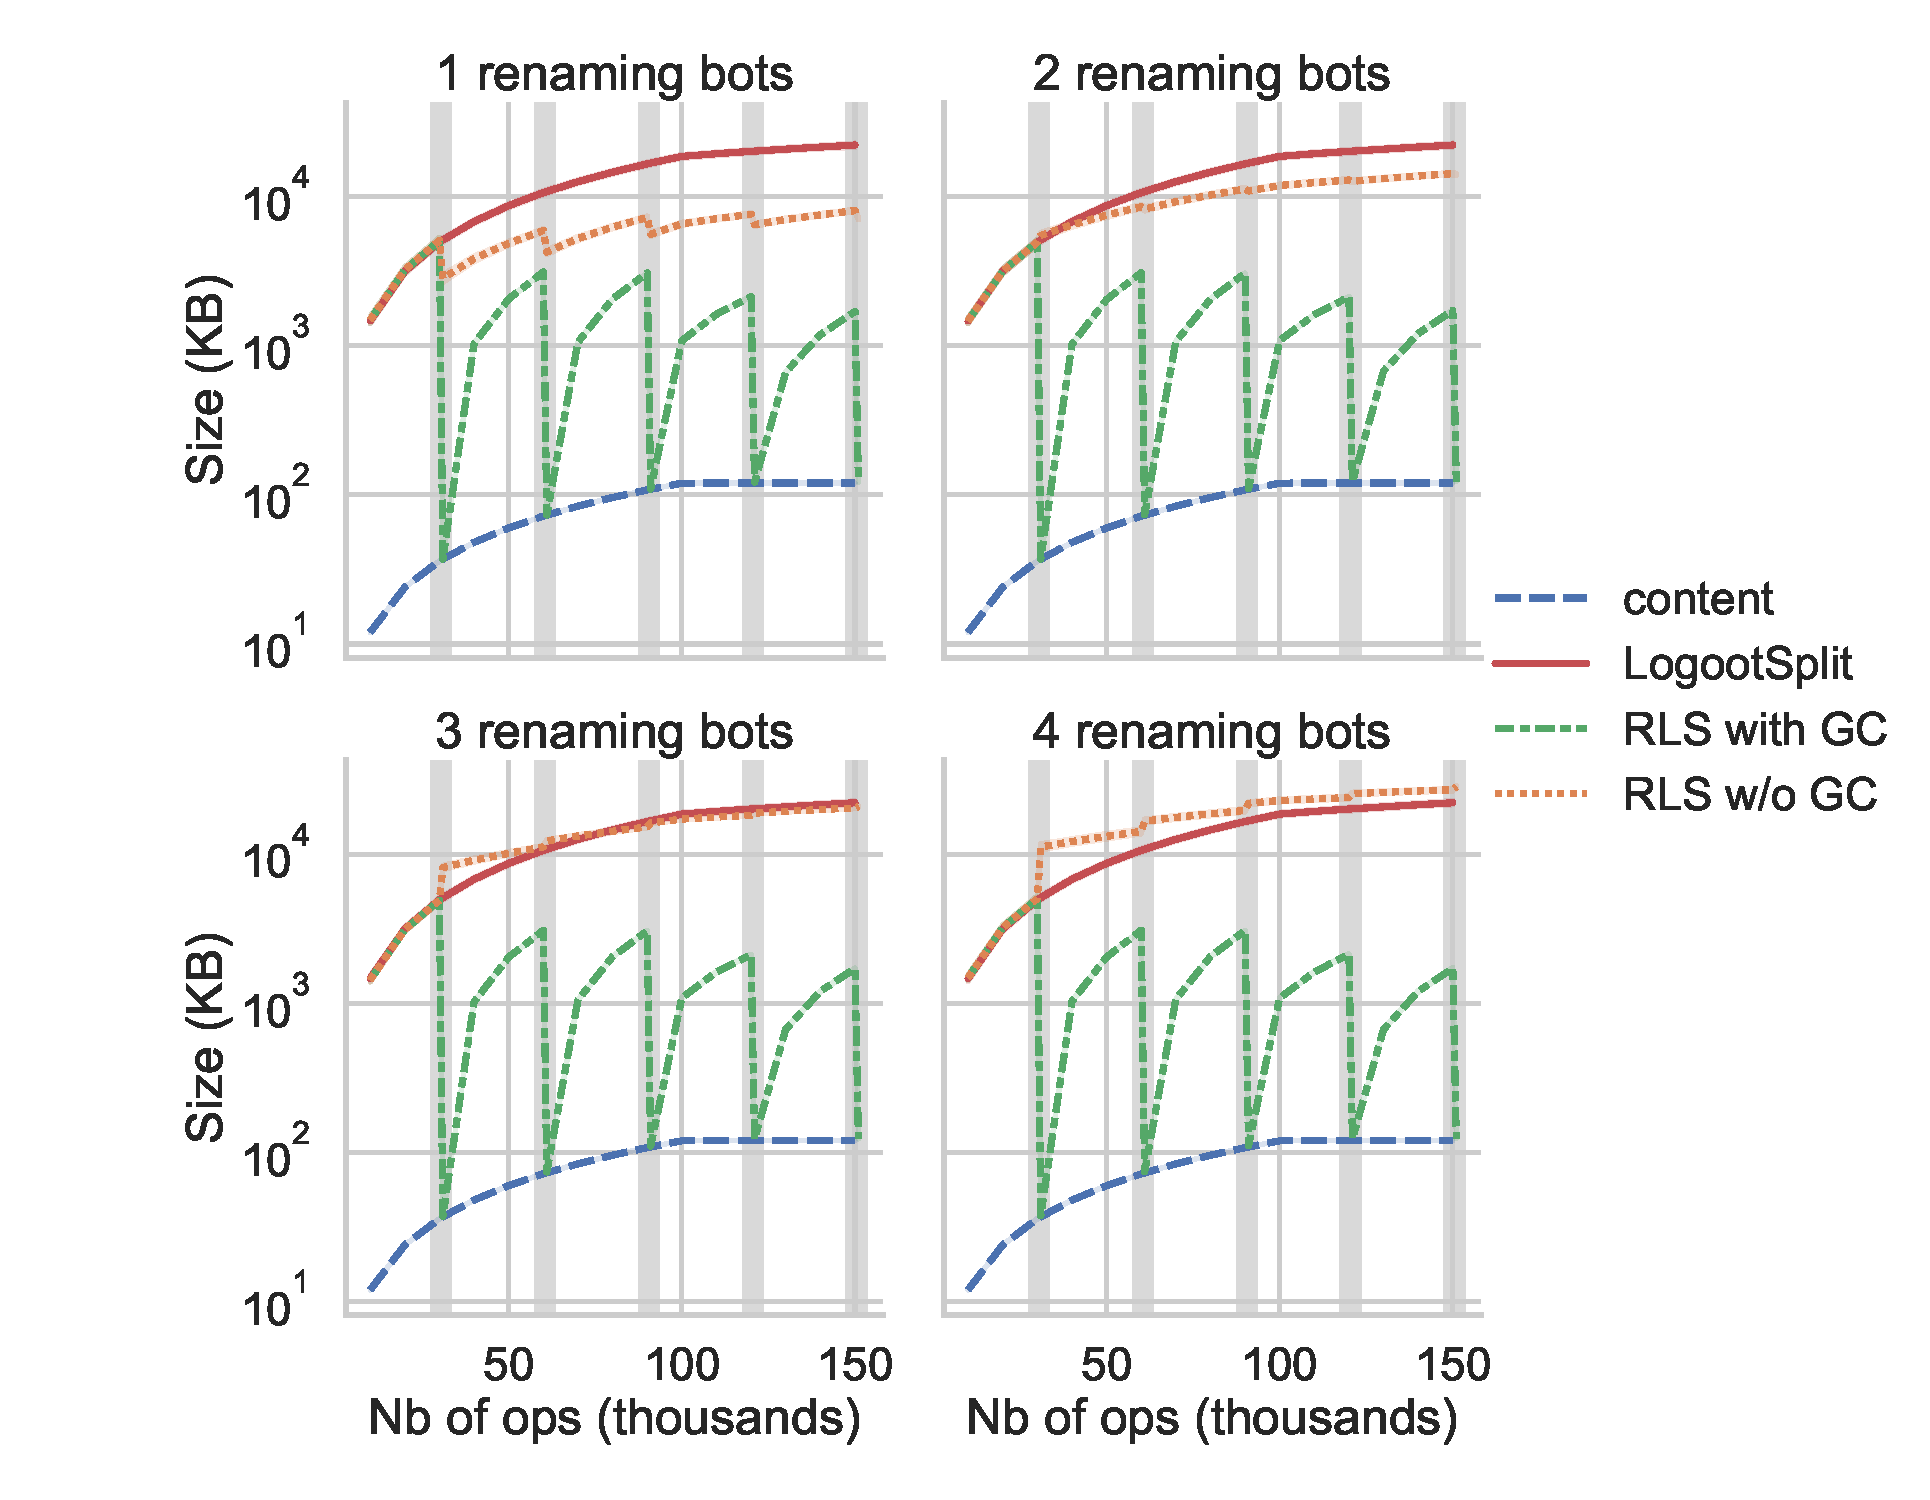
\includegraphics[width=\columnwidth]{img/snapshot-sizes.pdf}
    \caption{Evolution of the size of the document}
    \label{fig:evolution-document-size}
\end{figure}

For each plot displayed in \autoref{fig:evolution-document-size}, we represent 4 different data.
The blue dashed line illustrates the size of the actual content of the document, \ie the text, while the red solid line corresponds to the size of the whole LogootSplit document.

The green dashed-dotted line represents the size of the RenamableLogootSplit document in the best case scenario.
In this scenario, nodes assume that \emph{rename} operations are garbage-collectable as soon as they receive them.
Nodes are thus able to benefit the effects of the renaming mechanism while removing its own metadata, such as \emph{former states} and epochs.
In doing so, nodes are able to minimise periodically the metadata overhead of the data structure, independently of the number of \emph{renaming bots} and concurrent \emph{rename} operations issued.

On the other hand, the orange dotted line represents the size of the RenamableLogootSplit document in the worst case scenario.
In this scenario, nodes assume that \emph{rename} operations never become causally stable and can thus never be garbage-collected.
Nodes have to permanently store the metadata introduced by the renaming mechanism.
The performances of RenamableLogootSplit thus decrease as the number of \emph{renaming bots} and \emph{rename} operations issued increases.
Nonetheless, we observe that RenamableLogootSplit can outperform LogootSplit even in this worst case scenario while the number of \emph{renaming bots} remains low (1 or 2).
This result is explained by the fact that the renaming mechanism enables nodes to scrap the overhead of the internal data structure used to represent the document.

To summarise the results presented, the renaming mechanism introduces a temporary metadata overhead which increases with each \emph{rename} operations.
But the overhead will eventually subsides once the system becomes quiescent and \emph{rename} operations become causally stable.
In \autoref{sec:offloading-former-states}, we discuss that \emph{former states} may be offloaded until causal stability is achieved to address the temporary memory overhead.

\headerparagraph{Integration times of standard operations}
%
Next, we compared the evolution of integration times of standard operations, \ie \emph{insert} and \emph{remove} operations, on LogootSplit and RenamableLogootSplit documents.
Since both types of operation share the same time complexity, we used solely \emph{insert} ones in our benchmarks.
We do however distinguish \emph{local} and \emph{remote} updates.
Conceptually, local updates can be decomposed as presented in \cite{baquero2017pure} in the two following steps:
\begin{enumerate*}[label=(\roman*)]
    \item the generation of the corresponding operation
    \item the application of the resulting operation on the local replica.
\end{enumerate*}
However, for performance reasons, we merged these two steps in our implementation.
We thus make a distinction between \emph{local} and \emph{remote} updates in our benchmarks.
\autoref{fig:evolution-integration-time-insert} displays the results.

\begin{figure}[h!]
    \centering
    \subfloat[Local updates]{
        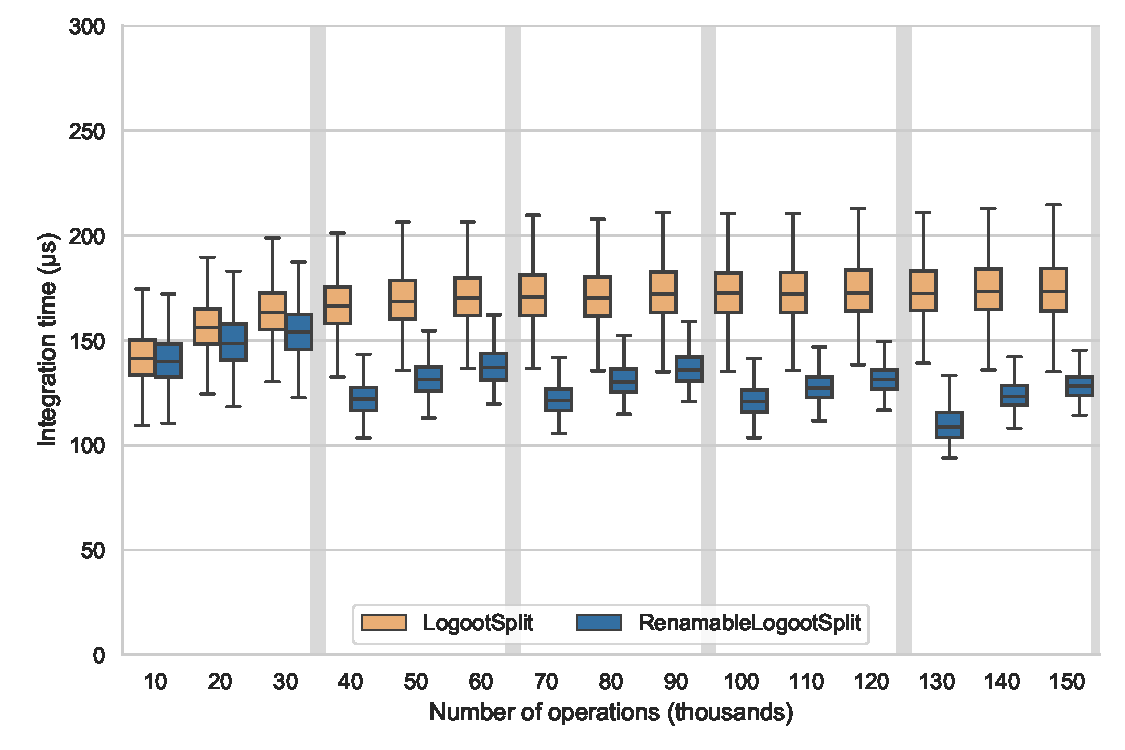
\includegraphics[width=0.9\columnwidth]{img/integration-time-boxplot-local-operations-without-outliers.pdf}
        \label{fig:evolution-integration-time-local-insert}}
    \hfil
    \subfloat[Remote updates]{
        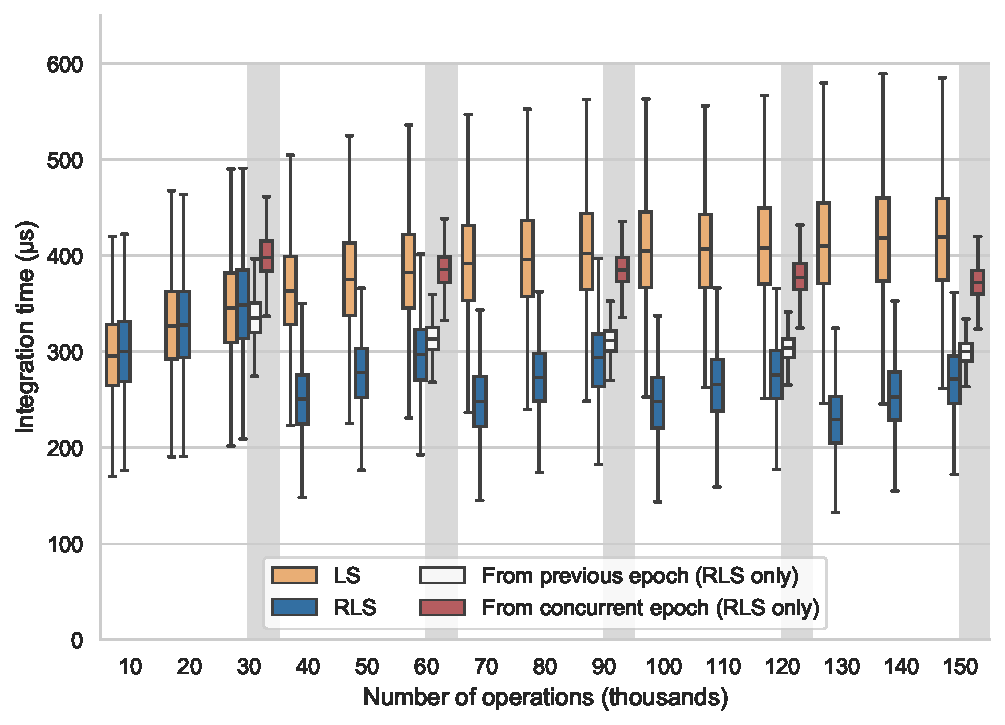
\includegraphics[width=0.9\columnwidth]{img/integration-time-boxplot-remote-operations-without-outliers.pdf}
        \label{fig:evolution-integration-time-remote-insert}}
    \caption{Integration time of standard operations}
    \label{fig:evolution-integration-time-insert}
\end{figure}

In these figures, orange boxplots correspond to integration times on LogootSplit documents while blue ones correspond to times on RenamableLogootSplit documents.
While both are initially equivalent, integration times on RenamableLogootSplit documents are then reduced when compared to LogootSplit ones once \emph{rename} operations have been applied.
This improvement is explained by the fact that \emph{rename} operations optimise the internal representation of the sequence.

Additionally, in the case of remote operations, we measured specific integration times for RenamableLogootSplit: integration times of remote operations from previous epochs and from concurrent epochs, respectively displayed as white and red boxplots in \autoref{fig:evolution-integration-time-remote-insert}.
Operations from previous epochs are operations generated concurrently to the \emph{rename} operation but applied after it.
Since the operation has to be transformed beforehand using \autoref{alg:renameId}, we observe a computational overhead compared to other operations.
But this overhead is actually compensated by the optimisation of the internal representation of the sequence performed by \emph{rename} operations.

Regarding operations from concurrent epochs, we observe an additional overhead as nodes have first to reverse the effect of the concurrent \emph{rename} operation using \autoref{alg:revertRenameId}.
Because of this overhead, RenamableLogootSplit's performances for these operations are comparable to LogootSplit ones.

To summarise, transformation functions introduce an overhead with regard to integration times of concurrent operations to \emph{rename} ones.
Despite this overhead, RenamableLogootSplit achieves better performances than LogootSplit as long as the distance between the epoch of generation of the operation and the current epoch of the node remains limited.
As the distance between both epochs increases, it leads to cases presenting worse performances than LogootSplit ones since the overhead is multiplied.
Nonetheless, the renaming mechanism reduces the integration times of the majority of operations, \ie the operations issued between two rounds of \emph{rename} operations.

\headerparagraph{Integration time of \emph{rename} operation}
%
Finally, we measured the evolution of integration times of \emph{rename} operation according to the number of operations since the last \emph{rename} one.
As before, we distinguish performances of \emph{local} and \emph{remote} updates.
The results are displayed in \autoref{tab:evolution-integration-time-rename}.

\begin{table}[t!]
    \centering
    \caption{Integration time of rename operations}
    \label{tab:evolution-integration-time-rename}
    \resizebox{\columnwidth}{!}{
        \begin{tabular}{lrrrrr}
            \toprule
            \multicolumn{2}{c}{Parameters} & \multicolumn{4}{c}{Integration Time (ms)} \\
            \cmidrule(lr){1-2} \cmidrule(lr){3-6}
            Type & Nb Ops (k) &   Mean &   Median & 99\textsuperscript{th} Quant. &    Std \\
            \midrule
            Local & 30  &    41.75 &    38.74 &      71.68 &   6.84 \\
                                    & 60  &    78.32 &    78.16 &      81.42 &   1.24 \\
                                    & 90  &   119.19 &   118.87 &     124.22 &   2.49 \\
                                    & 120 &   143.75 &   143.57 &     148.59 &   2.16 \\
                                    & 150 &   158.04 &   157.95 &     164.38 &   2.49 \\
            \cmidrule(lr){1-6}
            Remote & 30  &   481.32 &   477.13 &     537.30 &  17.11 \\
                                    & 60  &   981.62 &   978.24 &    1072.83 &  31.54 \\
                                    & 90  &  1491.28 &  1481.83 &    1657.58 &  51.10 \\
                                    & 120 &  1670.00 &  1663.85 &    1814.38 &  50.29 \\
                                    & 150 &  1694.17 &  1675.95 &    1852.55 &  59.94 \\
            \cmidrule(lr){1-6}
            Prim. Remote & 30  &   643.53 &   643.57 &     682.80 &  13.42 \\
                                    & 60  &  1317.66 &  1316.39 &    1399.55 &  28.67 \\
                                    & 90  &  1998.23 &  1994.08 &    2111.98 &  45.37 \\
                                    & 120 &  2239.71 &  2233.22 &    2368.45 &  50.06 \\
                                    & 150 &  2241.92 &  2233.61 &    2351.02 &  52.20 \\
            \cmidrule(lr){1-6}
            Sec. Remote & 30  &     1.36 &     1.30 &       3.53 &   0.37 \\
                                    & 60  &     2.82 &     2.69 &       4.85 &   0.45 \\
                                    & 90  &     4.45 &     4.23 &       5.81 &   0.71 \\
                                    & 120 &     5.33 &     5.10 &       8.78 &   0.90 \\
                                    & 150 &     5.53 &     5.26 &       8.70 &   0.79 \\
            \bottomrule
        \end{tabular}
    }
\end{table}

The main outcome of these measures shows that \emph{rename} operations are expensive when compared to others.
Local \emph{rename} operations take hundreds of milliseconds while remote ones and concurrent \emph{primary} ones may last seconds if delayed for too long.
It is thus necessary to take this result into account when designing strategies to trigger \emph{rename} operations to prevent them from impacting negatively user experiences.

Another interesting result from this benchmark is that concurrent \emph{secondary rename} operations are cheap to apply, as they only consist in storage of corresponding \emph{former states}.
Thus nodes can significantly reduce the overall computations of a set of concurrent \emph{rename} operations by applying them in a specific order.
We will discuss further this topic in \autoref{sec:postponing-transition-to-new-epoch}.

\section{Discussion}

\label{sec:discussion}

\subsection{Issuing \emph{rename} operations}
\label{sec:issuing-rename-operations}

As stated in \autoref{sec:definition-rename-operation}, \emph{rename} operations are system operations.
It is thus up to the designers of the system to determine when nodes should issue \emph{rename} operations and to define a corresponding strategy.
However, there is no silver bullet since each system has its own constraints.

Several aspects should be taken into account to define the strategy.
The first one is the size of the data structure.
As displayed in \autoref{fig:evolution-document-size}, metadata progressively increases to represent 99\% of the data structure.
Using \emph{rename} operations, nodes can discard metadata and reduce the size of the data structure to an acceptable amount.
To determine when to issue \emph{rename} operations, nodes may monitor the number of operations performed since the last \emph{rename} one, the number of blocks composing the sequence or the length of identifiers.

A second aspect to take into account is the integration time of \emph{rename} operations.
As reported in \autoref{tab:evolution-integration-time-rename}, integrating remote \emph{rename} operations takes up to seconds if delayed for too long.
Although \emph{rename} operations work behind the scenes, they can still impact negatively the user experience.
Indeed, nodes can not integrate operations from others while they are processing \emph{rename} operations
From users' points of view, \emph{rename} operations can thus be perceived as latency peaks.
In the domain of real-time collaborative editing, user experiments have shown that delay degrades the quality of collaborations \cite{ignat:hal-01088815,ignat:hal-01238831}.
It thus important to issue \emph{rename} operations frequently to keep their integration times below the perceptible limit.

Finally, the last aspect to consider is the amount of concurrent \emph{rename} operations.
\autoref{fig:evolution-document-size} shows that concurrent \emph{rename} operations decrease RenamableLogootSplit's performances.
The proposed strategy must then aim to minimise the number of concurrent \emph{rename} operations issued.
However, it should avoid to rely on synchronous coordination between nodes to do so.
To reduce the likelihood of issuing concurrent \emph{rename} operations, several techniques can be proposed.
For example, nodes can monitor to which other nodes they are currently connected and delegate to the one with the highest \emph{node identifier} the duty to issue \emph{rename} operations.

\subsection{Offloading on disk unused \emph{former states}}
\label{sec:offloading-former-states}

As explained in \autoref{sec:optimisations} and \autoref{sec:applying-primary-rename-op}, nodes have to store \emph{former states} corresponding to \emph{rename} operations to transform operations from previous or concurrent epochs.
Nodes may receive such operations given 2 different cases:
\begin{enumerate*}[label=(\roman*)]
    \item nodes have recently issued \emph{rename} operations
    \item nodes logged back in the collaboration.
\end{enumerate*}
Between these specific events, \emph{former states} are actually not needed to handle operations.

We can thus propose the following trade-off: to offload \emph{former states} on the disk until their next use or until they can be garbage collected.
It would enable nodes to mitigate the temporary memory overhead introduced by the renaming mechanism but increases integration times of operations requiring one of these \emph{former states}.
Nodes could adopt various strategies to deem \emph{former states} offloadable and to retrieve them preemptively according to their constraints.
The design of these strategies could be based on several heuristics: epochs of currently online nodes, number of nodes still able to issue concurrent operations, time elapsed since last use of the \emph{former state}...

\subsection{Designing a more effective \emph{priority} relation}
\label{sec:designing-more-effective-priority-relation}

Although the \emph{priority} relation proposed in \autoref{sec:priority} is simple and ensures that nodes designate the same epoch as the \emph{primary} one, it introduces a significant computational overhead in some cases.
Notably it allows a single node, disjoined from the collaboration since a long time, to force every other nodes to revert \emph{rename} operations they performed meanwhile because its own \emph{rename} operation is deemed as the \emph{primary} one.

The \emph{priority} relation should thus be designed to ensure convergence, but also to minimise the overall amount of computations performed by nodes of the system.
In order to design an efficient \emph{priority} relation, we could embed into \emph{rename} operations metrics that represent the state of the system and the accumulated work on the document (number of nodes currently at the \emph{parent} epoch, number of operations generated at the \emph{parent epoch}, length of the document...).
This way, we can favour the branch from the \emph{epoch tree} with the more and most active collaborators and prevent isolated nodes from overthrowing the existing order.

\subsection{Postponing transition to \emph{primary} epoch in case of high concurrency}
\label{sec:postponing-transition-to-new-epoch}

As shown in \autoref{tab:evolution-integration-time-rename}, integrating \emph{primary rename} operations is expensive as nodes have to browse and rename their whole current state.
This process can introduce a signification computational overhead in some cases.
Especially, a node may receive concurrent \emph{rename} operations in the reverse order to the one defined by the \emph{priority} relation.
In this scenario, the node would successively consider every \emph{rename} operation as the \emph{primary} one and would rename its state each time.
On the other hand \emph{secondary rename} operations are cheap to integrate, as nodes simply add to their state a reference to the corresponding \emph{former state}.

To mitigate the negative impact of this scenario, we can decompose the integration of \emph{rename} operations into two parts in case of concurrency detection.
First, nodes process \emph{rename} operations as secondary ones.
It enables nodes to integrate remote \emph{insert} and \emph{remove} operations, even from concurrent epochs, by transforming them.
Then each node keeps track of a level of confidence in the current \emph{primary} operation, computed for example from the time elapsed since the node received a concurrent \emph{rename} operation and the number of online nodes still known as using the \emph{parent} epoch.
Once the level of confidence reaches a given threshold, the node renames its state according to the operation.

This strategy introduces a slight computational overhead for each \emph{insert} or \emph{remove} operations received during the period of uncertainty, as nodes may issue operations from different epochs during that time.
In return, the strategy reduces the probability of erroneously integrating \emph{rename} operations as \emph{primary} ones.

\section{Related work}
\label{sec:related-work}

Several works were proposed to address our problem of growth of identifiers in variable-size identifiers Sequence \acp{CRDT}.
We present in this section the most relevant ones.

\subsection{The core-nebula approach}

The \emph{core-nebula} approach \cite{letia:hal-01248270, zawirski:hal-01248197} was proposed to reduce the size of identifiers in Treedoc\cite{5158449}, another variable-size identifiers Sequence \ac{CRDT}.

In this work, authors introduce a \emph{rebalance} operation enabling nodes to reassign shorter identifiers to elements of the document.
However, this \emph{rebalance} operation is not commutative with \emph{insert} and \emph{remove} operations nor with itself.
To achieve \ac{EC}\cite{10.1145/224057.224070}, the \emph{core-nebula} approach prevents concurrent \emph{rebalance} operations by regulating them using a consensus protocol.
Operations such as \emph{insert} and \emph{remove} can still be issued without coordination and can thus be concurrent to \emph{rebalance} ones.
To deal with this issue, authors propose a \emph{catch-up} protocol to transform these concurrent operations against the effects of \emph{rebalance} ones.

Since consensus protocols do not scale well, the \emph{core-nebula} approach proposes to split nodes among two groups: the \emph{core} and the \emph{nebula}.
The \emph{core} is a small set of stable and highly connected nodes while the \emph{nebula} is an unbounded set of dynamic nodes.
Only nodes from the \emph{core} participate in the execution of the consensus protocol.
Nodes from the \emph{nebula} can still contribute to the document by issuing \emph{insert} and \emph{remove} operations.

Our work can be seen as an extension of this work.
It adapts the \emph{rebalance} mechanism and the \emph{catch-up} protocol to LogootSplit and takes advantage of its block feature.
Furthermore, it integrates a mechanism to deal with concurrent \emph{rename} operations, hence removing the requirement of a consensus protocol.
It makes this approach usable in systems without existing authorities providing nodes to the \emph{core}.

However, systems can actually adopt the \emph{core-nebula} approach to simplify the implementation of RenamableLogootSplit.
The use of a consensus protocol to regulate \emph{rename} operations enables systems to discard all parts dedicated to the handling of concurrent \emph{rename} operations, \ie the design of a \emph{priority} relation and the implementation of \autoref{alg:revertRenameId} and \autoref{rule:gc-concurrent-primary-epoch}.

\subsection{The LSEQ approach}

The LSEQ approach \cite{lseq2013, lseq2017} is another approach proposed to address the growth of identifiers in variable-size identifiers Sequence \ac{CRDT}. Instead of reducing periodically the identifier metadata using an expensive renaming mechanism, the authors define new identifier allocation strategies to reduce their growth rate.

In this work, authors observe that the identifier allocation strategy proposed in Logoot\cite{WeissICDCS09} is suited to a single editing pattern: from left to right, top to bottom.
If insertions are made according to other patterns, generated identifiers quickly saturate the space of possible identifiers for a given size.
Following insertions therefore trigger an increase of the identifier size.
As a result, Logoot identifiers grow linearly with the number of insertions instead of the expected logarithmic progression.

LSEQ thus defines several identifier allocation strategy fitted to different editing pattern.
Nodes pick randomly one of these strategies for each identifier size.
Additionally LSEQ adopts an exponential tree model for identifiers: the range of possible identifiers doubles as the identifier size increases.
It enables LSEQ to fine-tune the size of identifiers according to needs.
By combining the different allocation strategies to the exponential tree model, LSEQ achieves a polylogarithmic growth of identifiers according to the number of insertions.

While the LSEQ approach reduces the growth rate of identifiers in variable-size identifier Sequence \ac{CRDT}, the sequence's overhead is still proportional to its number of elements.
On the other hand, RenamableLogootSplit's renaming mechanism enables to reduce metadata to a fixed amount, independently of the number of elements.

These two approaches are actually orthogonal and can, as in the previous approach, be combined.
The resulting system would reset the sequence's metadata periodically using \emph{rename} operations while LSEQ's identifier allocation strategies would reduce their growth in-between.
This would also enable to reduce the frequency of \emph{rename} operations, decreasing the system computations overall.

\section{Conclusions and future work}
\label{sec:conclusion}

In this paper, we introduced a novel Sequence \ac{CRDT} belonging to the variable-size identifiers approach: RenamableLogootSplit.
This new data structure embeds a renaming mechanism in its specification.
This mechanism enables nodes to reassign shorter identifiers to elements and to group them into one block to minimise metadata.
The renaming mechanism takes the form of \emph{rename} operations, system operations that are triggered automatically by nodes when deemed necessary.
However, the proposed \emph{rename} operation is not commutative with \emph{insert} and \emph{remove} operations, nor with itself.
Conflicts hence occur when operations are issued concurrently to \emph{rename} ones.
We thus described how RenamableLogootSplit adopts and uses \ac{OT} techniques to solve resulting conflicts.

We then presented the results of our empirical validation of RenamableLogootSplit through experiments.
Experiment results show that the renaming mechanism itself may temporary increase the metadata of the data structure, notably in case of concurrent \emph{rename} operations.
However the renaming mechanism enables nodes to garbage collect its own metadata eventually.
Nodes are thus able to reduce the size of their data structure by several hundred times compared to previous work eventually.

As future work, we will now focus on the design of strategies to manage the generation of \emph{rename} operations.
These strategies have to meet two different goals.
First, they have to minimise the impact of \emph{rename} operations on the user experience.
User behaviour studies, inspired by \cite{ignat:hal-01088815,ignat:hal-01238831}, could be led in the context of real-time collaborative writing to set an acceptable upper-bound to their integration times.
Strategies should then issue \emph{rename} operations accordingly to keep integration times below the defined threshold.
Secondly, strategies have to minimise the likelihood of issuing concurrent \emph{rename} operations without relying on consensus protocols.
Strategies should then use nodes' local knowledge to determine whether a node should issue a \emph{rename} operation or trust another node to do so.

Additionally, we would like to present a formal proof of the correctness of RenamableLogootSplit's algorithms.
Another research trail to explore is to study data types to determine which ones could benefit from a combination of \ac{OT} techniques and \ac{CRDT} ones for the design or improvement of their replicated counterpart.

% if have a single appendix:
%\appendix[Proof of the Zonklar Equations]
% or
%\appendix  % for no appendix heading
% do not use \section anymore after \appendix, only \section*
% is possibly needed

% use appendices with more than one appendix
% then use \section to start each appendix
% you must declare a \section before using any
% \subsection or using \label (\appendices by itself
% starts a section numbered zero.)
%


\appendices
\section{Algorithms for centralised settings}

\label{app:rename-id}

\begin{myalgorithm}[h!]
    \begin{algorithmic}
        \Function{renIdLessThanFirstId}{id, newFirstId}
        \If{id < newFirstId}
            \State \Return id
        \Else
            \State pos $\gets$ position(newFirstId)
            \State nId $\gets$ nodeId(newFirstId)
            \State nSeq $\gets$ nodeSeq(newFirstId)
            \State predNewFirstId $\gets$ \new~Id(pos, nId, nSeq, -1)
            \\
            \State \Return concat(predNewFirstId, id)
            \EndIf
        \EndFunction
        \\
        \Function{renIdGreaterThanLastId}{id, newLastId}
            \If{id < newLastId}
                \State \Return concat(newLastId, id)
            \Else
                \State \Return id
            \EndIf
        \EndFunction
    \end{algorithmic}
    \caption{Remaining algorithms to rename an identifier}
\end{myalgorithm}

% you can choose not to have a title for an appendix
% if you want by leaving the argument blank
\section{Algorithms for distributed settings}

\label{app:revert-rename-id}

\begin{myalgorithm}[h!]
    \begin{algorithmic}
        \Function{revRenIdLessThanNewFirstId}{id, firstId, newFirstId}
            \State predNewFirstId $\gets$ createIdFromBase(newFirstId, -1)
            \If{predNewFirstId < id}
                \State tail $\gets$ getTail(id, 1)
                \If{tail < firstId}
                    \State \Return tail
                \Else
                    \State offset $\gets$ getLastOffset(firstId)
                    \State predFirstId $\gets$ createIdFromBase(firstId, offset)
                    \State \Return concat(predFirstId, MAX\_TUPLE, tail)
                \EndIf
            \Else
                \State \Return id
            \EndIf
        \EndFunction
        \\
        \Function{revRenIdGreaterThanNewLastId}{id, lastId}
            \If{id < lastId}
                \State \Return concat(lastId, MIN\_TUPLE, id)
            \Else
                \State \Return id
            \EndIf
        \EndFunction
    \end{algorithmic}
    \caption{Remaining functions to revert an identifier renaming}
\end{myalgorithm}

\section*{Acknowledgments}

The authors would like to thank...


% Can use something like this to put references on a page
% by themselves when using endfloat and the captionsoff option.
\ifCLASSOPTIONcaptionsoff
  \newpage
\fi



% trigger a \newpage just before the given reference
% number - used to balance the columns on the last page
% adjust value as needed - may need to be readjusted if
% the document is modified later
%\IEEEtriggeratref{8}
% The "triggered" command can be changed if desired:
%\IEEEtriggercmd{\enlargethispage{-5in}}

% references section

\bibliographystyle{IEEEtran}
\bibliography{ref}

% biography section
%
% If you have an EPS/PDF photo (graphicx package needed) extra braces are
% needed around the contents of the optional argument to biography to prevent
% the LaTeX parser from getting confused when it sees the complicated
% \includegraphics command within an optional argument. (You could create
% your own custom macro containing the \includegraphics command to make things
% simpler here.)
%\begin{IEEEbiography}[{\includegraphics[width=1in,height=1.25in,clip,keepaspectratio]{mshell}}]{Michael Shell}
% or if you just want to reserve a space for a photo:

\begin{IEEEbiography}{Michael Shell}
Biography text here.
\end{IEEEbiography}

% if you will not have a photo at all:
\begin{IEEEbiographynophoto}{John Doe}
Biography text here.
\end{IEEEbiographynophoto}

% insert where needed to balance the two columns on the last page with
% biographies
%\newpage

\begin{IEEEbiographynophoto}{Jane Doe}
Biography text here.
\end{IEEEbiographynophoto}

% You can push biographies down or up by placing
% a \vfill before or after them. The appropriate
% use of \vfill depends on what kind of text is
% on the last page and whether or not the columns
% are being equalized.

%\vfill

% Can be used to pull up biographies so that the bottom of the last one
% is flush with the other column.
%\enlargethispage{-5in}

\end{document}
